%!TEX root=../tax-democracy-held.tex

\chapter[Wanted]{Wanted:\ Desirable and Doable Hypotheticals} \label{chap:wanted}

\begin{quote}
	\emph{``One should always look for a possible alternative, and provide against it.
It is the first rule of criminal investigation.''}\\*
	--- Sherlock Holmes in Conan \citeauthor{Doyle1904}'s \emph{The Adventure of Black Peter} \citeyearpar[567]{Doyle1904}
\end{quote}

In this crime story of the welfare state, tax and democracy, I follow Holmes' advise and attempt to rule out all possible alternatives.
The first alternative to be ruled out is --- counter-intuitively --- that, in Margaret Thatcher's words, \emph{there is no alternative}.
Before a criminal investigation of a corpse can begin in earnest, detectives have to show that it was not, in fact, a natural death.
Put another way, they must demonstrate that the deceased person \emph{might} have lived on, had not someone or something intervened.

To proceed by the method of elimination is always to conceive of such hypothetical outcomes, and then, to falsify them.
Still, hypotheticals
\footnote{
	By hypothetical, I mean an alternative state of the (\emph{dependent variable}) world.
	In history \citep[recently reviewed by][]{Bunzl2004} and political science \citep[for a methodological appraisal, see][]{Fearon1991}, the similar term \emph{``counterfactual''} sometimes refers to alternative (\emph{independent variable}) events in the past.
I ask what \emph{could be}, not what \emph{would be}.
}
are rarely invoked in social scientific explanations:
ever hear of an empirical sociologist or political scientist comparing the continental welfare state \citep{Esping-Andersen-1990-aa} or Westminster democracy \citep{Lijphart-1999-aa} to a \emph{non-existent} alternative?
We can see why few empirical social scientists would ask such a question:
to say that taxation could be more efficient and equitable, and to suspect that someone (for example, the rich) or something (for example, capitalism) is preventing it from being so reeks off conspiracy theory.

Forensics, in some ways, has it easier:
if a coroner diagnoses heart failure from old age as the cause of death, there is no murder.
If the autopsy reveals a coronary artery ruptured by a bullet, natural death is out of the question.

Just \emph{which} social ills are unavoidable and thereby the social scientific equivalents to a natural death is, unfortunately, more contentious.
Plausibly, without the bullet, an otherwise healthy person might have lived to see another day, but writ on a societal level, such hypothesizing about alternative, preferable outcomes is hard.
Would democracy \emph{not} always fall short of its ancient ideal, because we can no longer all meet and debate in person?
Would taxation \emph{not} always be wasteful, because it suppresses otherwise pareto-improving exchanges?
Would welfare \emph{not} always be a drag on growth, because it dampens incentives?

\begin{description}
	\item[Empiricism\phantomsection \label{itm:empiricism}]
	\emph{``We cannot know''}, might reply the empiricist \citep{Bacon1620,Locke1689,Hume1739} because such hypotheticals can, by definition, not be experienced with our senses and nothing can be induced from them.
%induce IS the correct word

	Whatever democracy, taxation and welfare \emph{could be}, we cannot know.

	Similarly, positivists might find these hypotheticals unknowable, either because absent, they \emph{have been} falsified \citep{Comte1842,Durkheim1895}, or, because absent, they \emph{cannot} be falsified \citep{Popper1934}.

	\item[Idealism \phantomsection \label{itm:idealism}]
	\emph{``We know only through ideas''}, might respond the idealists \citep[broadly][]{Kant1781,Hegel1807}, including the ideas invoked in these questions.

	Whatever democracy, taxation and welfare \emph{could be}, is beside the point, because our knowledge of them exists independent from their factual or hypothetical reality.

	Specifically, interpretive sociologists \citep{Weber1897} might argue that the above questions may contain in them already one of several, cultural perspectives, ideas or terminologies in which all answers, too, would be have to be phrased.
	``Waste'', ``growth'' and `incentives'' rather than objective things, already are cultural reality \citep[compare][]{Beland2010}.

	\item[Constructivism \phantomsection \label{itm:constructivism}]
	\emph{``Asks \emph{who}?''}, might retort the constructivist \citep{Berger1966,Paul1984}, because these are not questions about an objectively knowable world, but rather, the act of asking these questions and of invoking these concepts \emph{makes} that social world.

	Whatever democracy, taxation and welfare \emph{could be}, is beside the point, too, because legitimacy, efficiency, equity --- or any other criteria --- \emph{become} real, as we think, demand and reject them.

	\item[Rationalism \phantomsection \label{itm:rationalism}]
	\emph{``We can know''}, might announce the rationalists \citep{Descartes1637,Spinoza1662,Leibniz1704} --- \emph{``but hypothetical or actuality do not matter, either way''}.

	Whatever democracy, taxation and welfare \emph{could be}, we can know by deductive reasoning, without relying on our experience --- or absence thereof.
\end{description}

%I don't really take this stuff up again later.

%still missing
	%skepticism
	%disinterestedness

Clearly, \emph{none} of these epistemologies (or ontologies?) taken to the extreme, can help investigate those desirable, and doable hypotheticals upon which I have stumbled.
Welfare, taxation and democracy certainly are ideas, but they are also bound by empirics.
They are accessible to deductive reasoning, but such reasoning can make a social world, as much as it seeks to explain it.
What I need, is a \hyperref[sec:epistemology]{pragmatic and contingent middle way} (p.~\pageref{sec:epistemology}).
%maybe need more hrefs or otherwise refer to later discussion?

Equally clearly, such a cartoonish overview of epistemological traditions does not suffice to ground this dissertation.
Fortunately, this is --- as promised --- a pedestrian thesis and I will not abscond into any philosophy of science.
Unfortunately, I am also largely ignorant of these theories of knowledge, and can only provide a provisional epistemology that seems to work for democracy, taxation and welfare.

I take no pride in my epistemological ignorance, but I am weary of the obliviousness of these, and other meta-(meta?)-concerns.
In a slightly different context, Noam \citeauthor{Chomsky1997} has observed that ``ontological questions are generally beside the point, hardly more than a form of harassment'' \citeyearpar[132]{Chomsky1997}.
As harassments go, I have found that such epistemological and ontological debates often arouse what would appear to be deeply-felt passions in even the drowsiest of graduate seminars.
This fervor always struck me as eerily performative \cite[compare][]{Goffman1959,Butler1997}, as if, in addition to --- or as \emph{part of}
\footnote{
	Not to put too fine a point on it, but the language of these epistemological mudfights is conspicuously evocative of gender:
quantitative research is frequently referred to as \emph{hard} science, and qualitative and ideational approaches are often considered \emph{soft}, \emph{understanding} perspectives.
}
--- \emph{doing gender} \citep{West1987}, we were also \emph{doing social science}.

If only to stick to my limited last, I prefer a social science that serves people other than its researchers, and accordingly sympathize with pragmatist epistemologies, where human problems are primary and reified ``philosophical fallacies'' \citep{Dewey1929} take a back seat to the problems they were invented to solve.
%TODO pagenumber missing
In \citeauthor{Wikipedia2013}'s apt description of an (ecologically) pragmatist epistemology:
``inquiry is how organisms can get a grip on their environment" (retrieved in March 2013).

Even though, because hypotheticals are hardly invoked in the social sciences, are hard to specify, and are harder to know about I must devote this chapter to explicating the \hyperref[sec:epistemology]{epistemology} (p.~\pageref{sec:epistemology}), \hyperref[sec:axiology]{axiology} (p.~\pageref{sec:axiology}) and \hyperref[sec:ontology]{ontology} (p.~\pageref{sec:ontology}) of my research.

\section[Epistemology]{The Epistemology of Hypotheticals} \label{sec:epistemology}
\footnote{
	\label{fn:also-in-europe} This section is based, in part, on earlier, unpublished work which I submitted to the Hertie School of Governance in \cite{Held2012a}.
I have labelled said work as early drafts of this dissertation, and have since revised and expanded it.
}

\begin{quote}
	\emph{``If they can get you asking the wrong questions, they don't have to worry about the answers.''}\\*
	--- Thomas R.~Pynchon (*1937)
\end{quote}

Detective shows often confine the forensic medicine to some expository dialogue between coroner and inspector at the morgue.
I need a little more exposition here, stretching over several chapters of welfare economics, normative political theory and public choice, before the empirical action even begins.
Again, I merely proceed by the method of elimination.
To open an investigation, I must first know if there are alternative welfare states, taxes, and democracies out there, and if so, what they are.
%add appropriate hrefs

Surely, to suggest that we might learn something about the world by asking what is \emph{not} appears to be an odd epistemology.
Natural scientists probably do not spend much time thinking up, say, a counterfactual universe without gravity, and explaining why it is not (or maybe that \emph{is} what they do at the Large Hadron Collider?!).
Positive social science, at least, needs to pose these why-not-questions, because, unlike physics, it is concerned with \emph{who} or \emph{what} made the world the way it \emph{is}
\footnote{
	Physicist \citet{Krauss2012} has pointed out that strictly speaking, \emph{why} questions are teleological:
they imply purpose.
	Positive social science --- as physics --- need not assume such purpose, and therefore better ask \emph{how} questions.
	I use the two interchangeably.
}.

Positive sociology, political science, and this dissertation, all ask such second-order questions.
Even to pose them, we need all the possible first-order answers of how the world \emph{could} be, but is not.
The hypotheticals I establish in the following chapters are these first-order \emph{non}-answers.

\subsection{First-Order Questions \label{sec:1st-questions}}
Hypotheticals must be \hyperref[sec:ontology]{\emph{materially doable}} (p.~\pageref{sec:ontology}), and --- if you allow some humanist bias --- they must also be at least somewhat \hyperref[sec:axiology]{\emph{normatively desirable}} (p.~\pageref{sec:axiology}).
Those criteria both raise inquiries of the first order, asking what is normatively good and what is positively possible, respectively.

% ``A great deal of work on deliberative theory focuses on conflicting values, religious toleration, identities and so on, and relatively little on conflicting facts.'' \cite[2]{Moore2011}
\emph{Normative} (or prescriptive) social science asks such first-order questions as how to emancipate people (critical theory, maybe from \citeauthor{Gramsci1971}  to \citeauthor{Adorno-1974-aa}, Horkheimer and \citeauthor{Habermas-1984}), what makes rule legitimate (political theory from \citeauthor{Aristoteles} to \citeauthor{Dahl-1989-aa}) or what allocation might be fair (distributive justice including \citeauthor{Friedman1962} and \citeauthor{Rawls1986}) and even what makes an economy rich (economics from \citeauthor{Smith-1776-lq} to \citeauthor{Hicks1939}).
Even these apparently normative and first-order questions turn into positive and second-order questions when their underlying assumptions on human nature are tested or problematized, respectively (more on that \hyperref[itm:constructivism]{constructivist} twist on p.~\pageref{itm:constructivism}).

\emph{Positive} social science asks few, if any, first-order questions, because as it asks about the social world (for example, health insurance), it seeks to explain the social conflict of \emph{answering} a first-order question (for example, how to spread risk).
To the extent that nominally \emph{social} sciences have carved out positive research agendas of the first order (for example, cognitive psychology, behavioral economics), they cease to be social science but revert to a natural science of some ideally \emph{physically} rooted phenomenon (for example, neuroscience).
Tautologically, if the social sciences are to be concerned with explaining social choice, they know \emph{no} positive first-order questions, because first-order status negates choice
\footnote{
	To deny such social choice, and to \hyperref[chap:hypotheticals-matter]{reduce social science to purported positive first-order questions} easily feeds into an ideological affirmation of the status quo (\autoref{chap:hypotheticals-matter}, p.~\pageref{chap:hypotheticals-matter}).%update href
}.

The aspects of the social world under study here are welfare, taxation and democracy.
To the extent that these social choices hinge on last reasons, they raise normative first-order questions.
These first-order questions of efficiency and equity, fairness and legitimacy have been widely discussed, and I will reference them only briefly in this dissertation.
%add hrefs

But welfare, taxation and democracy also raise two kinds of positive questions
\footnote{
	Formal logic and empirical finding are not as neatly divided as I make them out to be.
	Frequently, formal models generate the hypotheses that empirical works set out to falsify.
	Conversely, inconsistent empirical findings inspire new, better formal modeling.

	Still, in the way of this boundary-blurring also lie ad-hoc fallacies.
	When formal logic and empirical finding become too closely enmeshed, the resulting hypotheses may become unfalsifiable.
	\cite{Popper1976} has thus criticized (some) Darwinism for being unfalsifiable, because any possible observed biological trait must, tautologically, have been adaptive for otherwise it could not have survived --- a critique that has since been (mis)appropriated by creationists.

	More relevant here, much of the modern infatuation (and outrage) with general equilibrium economics, might be explained by a similar, unhappy but popular conflation of brilliant formal logic \citep{Walras1874,Debreu1954} with murky assumptions on human nature on which that logic supposedly operates, thereby morphing equilibrium economics from tentative model to hermetic ideology (\citealt{Cassidy2010} tells the entire, sad story).
}
:

\begin{description}
	\item[A Priori Knowledge \phantomsection \label{itm:a-priori}]
	There may only be finite or even unique ways to organize these institutions that abide by \emph{formal logic}, per reasoned, \emph{a priori knowledge}.

	For example, a welfare state financed solely by printing money may be an economically illogical institution (possibly resulting hyperinflation resembles a pyramid scheme).
	Similarly, taxing judicial persons, such as corporations, may be economically nonsensical because such organizations are no moral subjects and the incidence would be arbitrary (\autoref{chap:doable-tax}).
%improve href
	As a last example, a democratic aggregation mechanism may not be able to maximize both majority rule and proportional representation, simply because the two criteria conflict.

	Knowledge about what is logically possible or impossible flows from a \hyperref[itm:rationalism]{rationalist} epistemology (p.~\pageref{itm:rationalism}).

	\item[A Posteriori Knowledge \phantomsection \label{itm:a-posteriori}]
	These formally logical designs may be further limited by empirical, first-order findings on human nature or other material conditions, per experiential, \emph{a posteriori} knowledge.

	For example, a welfare state financed by extracting and burning fossil fuels may soon run into physical constraints if we observe limited resources and related global warming.
	Similarly, a fully-planned economy (instead of taxation) may, amongst other things, dramatically overestimate the cognitive ability of human planners to centrally aggregate and process dispersed information.
	Lastly, a democracy modeled on ancient Athens, but with universal suffrage and in globally integrated economies may fail simply because human beings interact too slowly to listen to every fellow human on the planet, let alone to get anything done
	\footnote{
		Also, wryly observe \citeauthor{GutmannThompson-2004-aa}, ``for most people, the freedom not to spend a major part of one's time deiberating about politics is part of what it means to live the life of a free citizen'' \citeyearpar[30]{GutmannThompson-2004-aa}.
	}.

	Knowledge about what is empirically possible or impossible flows from an \hyperref[itm:empiricism]{empiricist} epistemology (p.~\pageref{itm:empiricism}).
\end{description}

These are, admittedly, uncontroversial constraints and ludicrous suggestions --- I want to keep the more interesting problems for later --- but they illustrate an important point:
there probably \emph{are} some first-order, positive limits the social world faces, even though we may know little and disagree a lot about them.

Crucially, we may disagree on whether a given question is of the first or second order.
The social sciences, in particular, have a habit of reassigning first-order questions to second-order status:
\emph{that} is the project of constructivism \citep[for example,][]{Berger1966} and \hyperref[itm:constructivism]{related epistemologies} (p.~\pageref{itm:constructivism}) to see social phenomena not as ``things \emph{in} the world, but perspectives \emph{on} the world'' \citep[174 on ethnicity, emphasis in the original]{Brubaker-2002-aa} or as contested and consequential second-order \emph{answers}.
Still, even a die-hard idealist or constructivist may concede some irreducibly positive, first-order questions, and to those, the social sciences offer no answers.

So it is with welfare, taxation and democracy.
Their design probably faces some --- albeit uncertain and contested --- positive limits of the first order.
To ask about these limits is, emphatically, \emph{not} a question for the social sciences.
Instead, \emph{nominally} social scientific, but formally mathematical-logical disciplines such as equilibrium economics
\footnote{
	I assume economic production to be approximately described by mainstream (neoclassical?) textbook economics \citep[including][]{Mankiw-2004-aa,FrankBernanke2004}, expanded by some ventures into welfare economics \citep{Hicks1939,Samuelson-1954-eu},  game theory (founded by \citealt{VonNeumannMorgenstern1944,Nash1951},  expanded by \citealt{Axelrod1981a}, recently summarized by \citealt{Kleinberg-2009-oz}) and network theory (for example, \citealt{Mandelbrot2004}, \citealt{Jackson1968} also recently summarized by \citealt{Kleinberg-2009-oz}).
}
and public choice ask about the \hyperref[itm:internal-consistency]{internal consistency} of such societal institutions, based on assumptions on \hyperref[itm:a-posteriori]{human and other nature} (p.~\pageref{itm:a-posteriori}), which are in turn hypothesized and falsified by such natural sciences as evolutionary psychology (a.k.a.\ sociobiology), social psychology \citep[initially][]{KahnemanTversky1979}, cognitive science, or even physics.
I suggest two examples of such first-order, positive substrates relevant to my subject matter:
\begin{enumerate}
	\item
	The first theorem of welfare economics is often invoked as a first-order constraint on welfare state interventions or taxation (the \gls{DWL}), and it also shines through in some radical defenses of pluralist democracy \citep[for example,][]{Caplan2007}.
	The theorem states that over any \emph{given} distribution, free competition equilibrates at pareto optimality
	\footnote{
		Demonstrated first graphically by \cite{Lerner1944}, mathematically by \cite{Lange1934}, \cite{Debreu1954} and others.
	}
	and that therefore, no allocative intervention can make anyone better off without making someone else worse off.
	It is a mathematically formulated argument about some internal consistency of the market mechanism:
given certain \hyperref[sec:perfect-competition]{(heroic) assumptions} (p.~\pageref{sec:perfect-competition}), market equilibria \emph{cannot} be pareto-improved.

	As such, the theorem is just that, an exercise in formal logic, not more:
not empirical claim (no ``proof'' that \emph{actual} markets pareto-optimize) and not normative statement (no justification for pareto-optimization over existing distributions as desirable).
	But the first theorem is also not less:
properly understood, it \emph{is} a first-order constraint and invites \emph{no} second-order critique.

	\item
	Similarly, homo economicus is often invoked in the field of welfare (\emph{``knaves''} as in \citealt{LeGrand2003}), taxation (\emph{``people react to incentives''} as in \citealt[24]{Mankiw-2004-aa}) and democracy (\emph{``rationally irrational''} as in \citealt{Caplan2007}).
	The concept implies that human beings make rational, self-interested and utility-maximizing decisions (maybe first \citeauthor{Mill1848}, \citeauthor{Smith-1776-lq}, recently including \citealt{Robbins1976} on rational choice, all summarized in \citealt{Persky1995}).
	The ideological campaign (and backlash) wrought by homo economicus and its offspring notwithstanding, it is, properly understood, merely a \emph{falsifiable}
	\footnote{
		And falsified, it has been:
for example, \cite{Alvard2004} on fairness, not utility, \cite{Zak2004a} on reciprocity, not self-interest, \cite{KahnemanEtAl1982} and \cite{Simon-2001-aa} on biased and bounded, not complete rationality.
	}
	assumption about human nature that welfare, taxation and democracy might have to heed if it were, in fact, correct.
	But even if it were true, homo economicus would be just that, an empirically verified model:
no more (no normative claim of how we \emph{should} be), but also no less (no socially contingent phenomenon in need of deconstruction).
\end{enumerate}

\subsection{Second-Order Questions \label{sec:2nd-questions}}
As forensics informs a criminal investigation, the first-order answers provide the reference for the second order inquiries.
These ask who or what decides first-order answers, or, metaphorically, who or what brought about the observed forensic outcome (see \autoref{tab:1st-2nd-order-questions}, p.~\pageref{tab:1st-2nd-order-questions}).
Second-order inquiries seek to criticize, explain or test the \emph{social conflict} over first-order questions.

Social science asks plenty of those questions on welfare, taxation and democracy.

It asks, for example, why and how welfare states --- a first-order \emph{answer} --- evolve(d):
because modernization replaced inherited, familial status with citizenship and the market \citep{Titmuss1974,Marshall-1950-aa}, because industrialization required an appeased, reliable and healthy workforce \citep{Flora1981,Wilensky1975}, because workers gained power \citep{Korpi1983,Jessop2002}, because institutions prevail \citep[for example,][]{Rothstein}, because ideas matter \citep[for example,][]{Stiller2009} because initial class cleavages lead to different degrees of commodification \citep{Esping-Andersen-1990-aa} or because capitalism comes in variants \citep{HallSoskice-2001-aa}
\footnote{
	For a good overview of social theories of the welfare state, see \cite{BrooksManza2007} %this appears to be the wrong citation, some screwup with the citecode suggests that originally I meant something by Beland 2008, not in mendeley
	.
}.

So it is with the second-order theories of taxation:
it arose as proto-states extracted the resources enabled by, and necessary for greater economies of scale in their state-making and war-making \citep{Tilly-1985-aa}, it (sometimes) erodes to lower levels as internationally mobile factors of production and consumption arbitrage over different national rates (recently reviewed in \citealt{Genschel2010}), it persists at similar levels as domestic politics prevents roll-back \citep{Swank2002}, or it changes bases and schedule in response to these pressures \citep{Kemmerling2009}.
 %need more general literature here, not this contentious one-sided stuff, maybe more from the fiscal sociology stuff.

And so, too, it is with the second-order theory of pluralist democracy:
states introduced popular rule, because the costs of otherwise considered illegitimate extraction became prohibitive \citep{Tilly2006}, democracy belongs to a broader syndrome of emancipating modernization, including a market economy and corresponding rational and self-expression values \citep{InglehartWelzel-2005-aa} or the sequential development of citizenship (instead of other, pre-modern statuses) entailed democratic rights \citep{Marshall-1950-aa}.
%need more general literature here

These are variations on the questions of sociology:
what binds us together (social integration), and what keeps us apart (social inequality
\footnote{
	The first question of sociology, according to \citet[66]{Dahrendorf1966}.
}).
These are also the questions of political science:
how do power, norms, ideas and institutions rule human interactions?
These second-order questions are open to all epistemologies, including the the anti-positivist traditions of \hyperref[itm:idealism]{idealism} and \hyperref[itm:constructivism]{constructivism}.
They can also be --- as seems to be currently en vogue
\footnote{
	In 2012, a political scientist, paraphrasing \cite{Wittgenstein1998}, described the current expectations in German political sciences to me thus:
``whereof one cannot measure, thereof one must be silent''.
 %ask for permission to quote genschel

	The same political scientist also opined --- maybe slightly in-jest -- that ``excellence is finishing on time'', referring to the \gls{BIGSSS} application for federal excellence initiative funding.
}
---, \emph{but need not be}, entirely  \hyperref[itm:empiricism]{empiricist} or, \hyperref[itm:rationalism]{rationalist} inquiries.

And important questions, they are, asking us, that lone ``hypercultural'' species \citep{Henrich2004}, how we make our own history.
In our rich time and in our unequal place, welfare, taxation and democracy may just be \emph{the} historical battlegrounds, on which these sociological and political forces operate.

This dissertation develops a second-order theory of social change to explain the defeats these institutions have suffered in late capitalism, and tests it empirically
\footnote{
	For the distinction between first-order and second order questions, I am indebted to Claus Offe, who first suggested I should develop a second-order theory of social conflict on tax choice.
}.

\begin{table}[htbp]
	\centering
	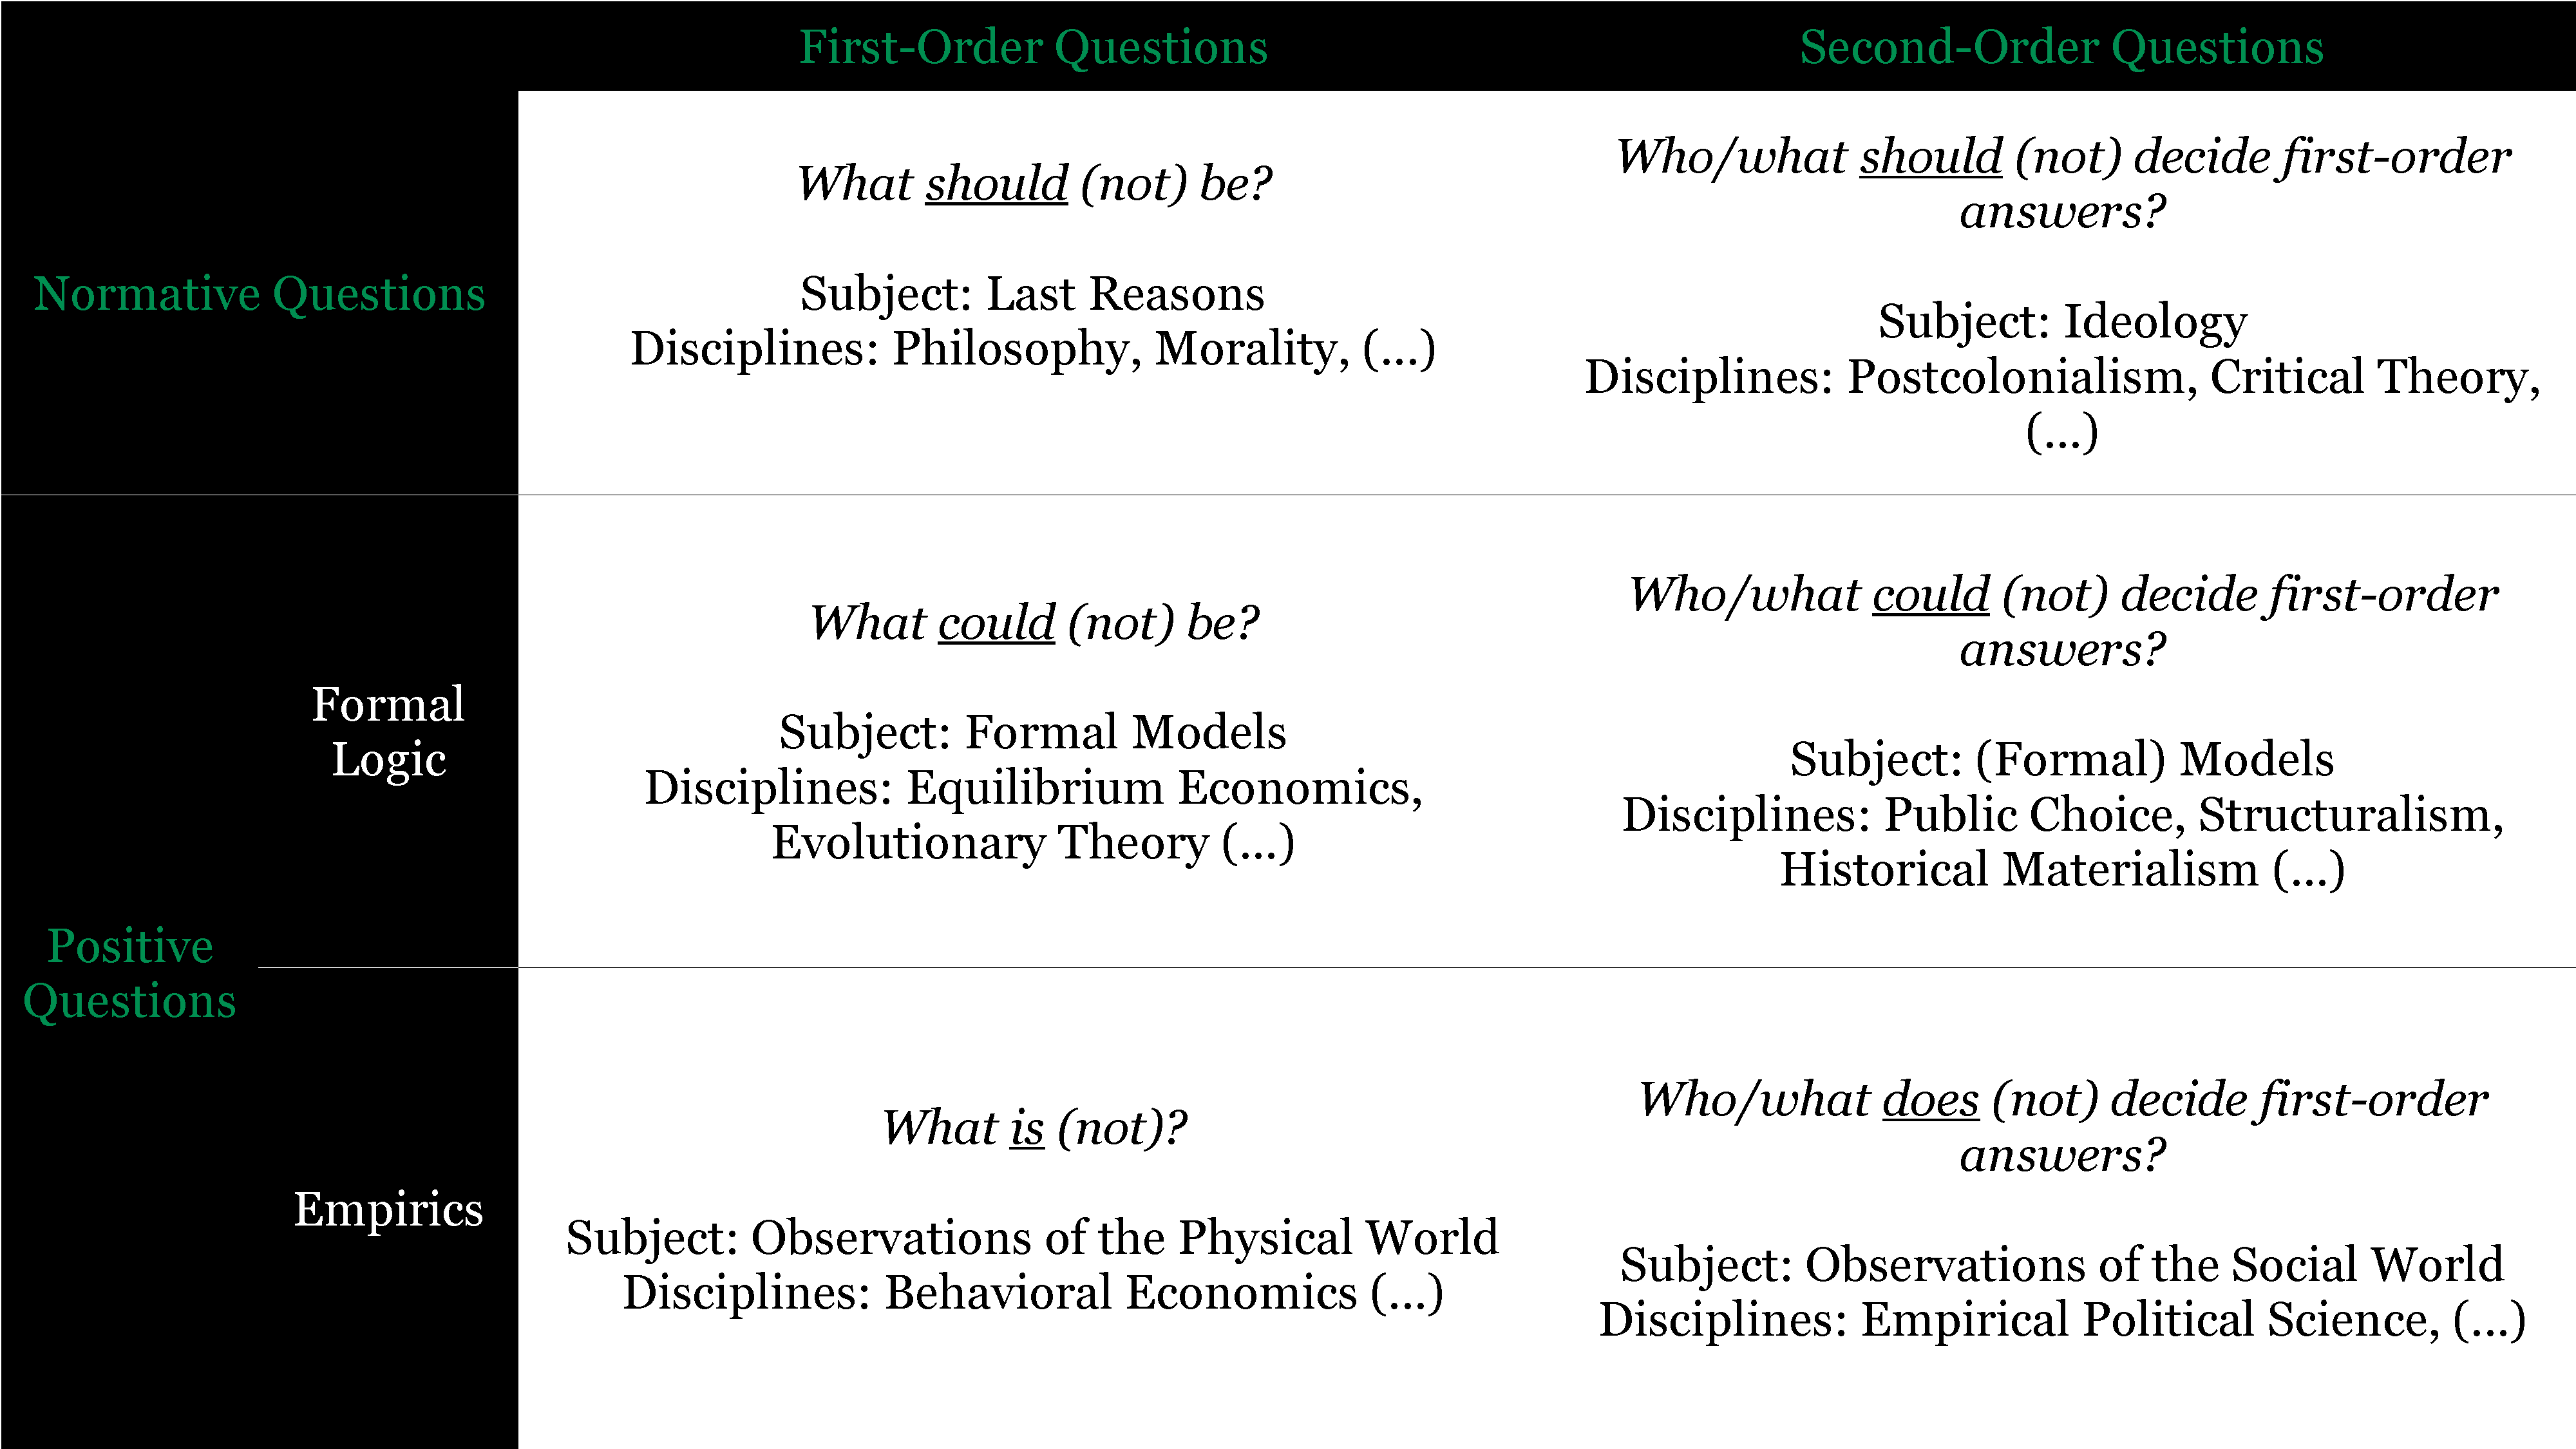
\includegraphics[width=1\linewidth]{orders-of-questions}
	\caption{Overview of First, Second-Order, Normative and Positive Questions}
	\label{tab:1st-2nd-order-questions}
\end{table}

The distinction between first-, second-order, normative and positive questions summarized in \autoref{tab:1st-2nd-order-questions} (p.~\pageref{tab:1st-2nd-order-questions}) matters for at least two reasons:

\begin{enumerate}
	\item
	Clearly addressing one of these questions at a time, and striving to keep them separate makes for better social science.
	With these categorically different questions come different goals, languages and methods.
With blurring or negating these categories come ``politics-based evidence making'' (The Economist 2012), apolitical ignorance or both.
	\item
	Because positive social science --- including this dissertation --- is out to explain the second-order decision on first-order questions, it must consider some first-order theory \emph{first}.
\end{enumerate}

\subsection{First Order Theory \emph{First} \label{sec:1st-questions-first}}
I am ultimately interested in the second-order questions of welfare, taxation and democracy, but proceeding by the method of elimination, I must first ask and answer the first-order questions:
what \emph{should} and \emph{could} welfare, taxation and democracy look like.

Consider the two alternatives, that I must rule out before any second-order questions can be raised:

\begin{description}
	\item[No Desirable Hypothetical.]
	If I could find only the presently observed design of welfare, tax and democracy to be at least somewhat desirable, there would be no social conflict to be explained, much like there is no need for a political science of wearing sunscreen.
	(I partly take this \hyperref[sec:axiology]{later}, p.~\pageref{sec:axiology}).

	In the crime story metaphor, if the corpse in question had previously run amok shooting innocents, rupturing that persons coronary artery with a bullet might be have been self-defense or the last resort, and the only desirable course of action.
	No \emph{further} criminal investigation may be necessary.

	\item[No Doable Hypothetical.]
	If I could find only the presently observed design of tax and democracy to be materially doable, there would be no social conflict to be explained, much like there is no need for a sociological theory of gravity.
	%here, too:
%I partly take this back later \ldots

	In the crime story metaphor, if said deceased suffered from an irreparable birth defect that caused the heart failure, no outcome but death is materially possible.
	In that case, too, no criminal investigation will be necessary.
\end{description}
%add table here to further explain these.
%crosstab it.

Conceiving such to-be-ruled-out hypotheticals raises normative (desirability) and positive (doability) questions of the \emph{first}-order.
These first-order questions cannot, as I explained above, be answered by social sciences (alone), but I must instead reference other disciplines, much like a detective hears forensic evidence.

If these ancillary disciplines reveal one, or several such desirable and doable hypotheticals that I cannot rule out, the non-occurrence of such hypothetical welfare, taxation and democracy beg a second-order explanation just as the observed arrangement requires explanation.
In fact, the two are the same thing:
to explain the presence of the present arrangement is to explain the absence of all absent arrangements.

For illustration, consider the inverse scenario, in which I find no desirable and doable hypotheticals in welfare, taxation and democracy.
If that were the case, there would be no second-order decision to be explained, because without such hypotheticals, there is no human choice.

If however, there \emph{are} desirable and doable hypotheticals, any second-order question always invokes these hypotheticals.

\subsection{Fallacies and Risks}
%better title:
%glass full empty?
To be sure, this reasoning is not logically watertight and might turn into an argument from ignorance:
even if I find no reason why hypotheticals should, or could not be, they might still be undesirable or impossible for some other reason.
Absence of evidence, here, too, does not constitute evidence of absence.

The same problem must plague medical forensics:
no evidence of natural death does not prove a violent death and any conclusion to the contrary might cause an unnecessary murder investigation.
In practice, this possible fallacy simply raises the question of where you place the burden of proof, because you can err either way:
if you take absence of evidence of violent death as evidence of natural death, you might foreclose a necessary investigation and let someone get away with murder.
Tellingly, when it comes to human corpses we place the burden of proof on the status quo:
if the cause of death cannot be established --- if there is \emph{no} evidence of natural death --- the prosecution customarily opens an investigation.%find source for this

The positive social science of welfare, tax and democracy seems to have adopted a somewhat laxer standard.
Here, much empirical work implicitly places the burden of proof on the hypothetical:
without evidence that the hypothetical is normatively desirable and materially possible, the fundamental status quo of welfare and tax needs no social explanation.
Conveniently, as hypotheticals go, they rarely produce conclusive evidence of their desirability and doability.
Maybe, this is just the skepticism that positivism calls for --- or maybe, \hyperref[chap:hypotheticals-matter]{hypotheticals matter}, and such social science invariable turns latently affirmative (\autoref{chap:hypotheticals-matter}, p.~\pageref{chap:hypotheticals-matter}).

Either way, I here place the burden of proof on the status quo.
If I find no reasons to the contrary, I assume that there \emph{are} several doable and desirable designs of tax and democracy, and require social science to explain the \emph{absence} of all but the presently observed design.
If we apply the standard of forensics, any second-order theory of social change must be able to explain how the social conflict under study resulted in the non-occurrence of these alternative designs, especially the attractive ones.

I still want to shoulder part of the burden of proof.
In tax, I can only plausibilize the hypotheticals by reviewing reputable work by others, and deduce my case from reasonable assumptions about human nature, and the economy.
I must rely mostly on a \hyperref[itm:rationalism]{rationalist} epistemology (p.~\pageref{itm:rationalism}).
Natural experiments --- the \hyperref[itm:empiricism]{empiricist} gold standard --- are unavailable, and all others suffer from limited external validity:
a modern economy does not fit in the laboratory and equilibrium simulations poorly model such inframarginal institutional changes.
%more on this somewhere else.
%Should explain why I can't look into tax in another way! Reference this section here.
In democracy, I similarly plausibilize the hypotheticals, but I can also point to and undertake some preliminary experimental tests.

To suggest, as I do, that there are desirable and doable hypotheticals in tax and democracy, must remain a preliminary proposition open to falsification.
To the \citeauthor{Popper1934}ian scientist, there is always some absence of evidence, and therefore, no evidence of absence.
If these particular hypotheticals turn out to be undesirable or impossible, so collapses any second-order hypothesis I might wager later, but, I hope, we will still have learned something.

Not only the advancement of science depends on such falsification, the history of progressive causes is also littered with what might charitably be called ``false positives''.
My chosen hypotheticals --- deliberative democracy and progressive taxation of (unimproved) land value and (postpaid) consumption, too, may inspire such false hopes.
They, too, should be approached with great care, especially, when they necessitate constitutional or otherwise reform of liberal democracy, as deliberative democracy may one day do.
Tax reform, at least, should be open to falsification and is not an end in itself, especially because it thoroughly hinges on economic contexts and human motivation.
%or maybe, deliberation is an end in itself, as a school for democracy

Then again, by any historical standard --- once-hypotheticals failed (for example, socialism) and successful (for example, universal suffrage) alike --- here are some fairly incremental reforms as carefully liberal in their \hyperref[sec:axiology]{normative axioms} (p.~\pageref{sec:axiology}) as they are conservative about \hyperref[sec:ontology]{ontological possibilities} (p.~\pageref{sec:ontology}).

\section[Axiology]{Axioms for Desirable Hypotheticals} \label{sec:axiology} %or last reasons?

\begin{quote}
	\emph{``I believe in clear-cut positions.
I think that the most arrogant position is this apparent, multidisciplinary modesty of \emph{`what I am saying now is not unconditional, it is just a hypothesis,'} and so on.
[\ldots] I think that the only way to be honest and expose yourself to criticism is to state clearly and dogmatically where you are.
You must take the risk and have a position.''}\\
	--- Slavov \citet[45]{Zizek2003}
\end{quote}

Normatively desirable hypotheticals are preferable to others if we assume a basic humanist, or critical intention of positive social science and policy analysis to improve human lives.

From a strictly positivist point of view, this is the flimsiest of epistemological decisions I take:
we might learn just as much about the social world from the nonoccurrence of bad outcomes, as from the nonoccurence of good outcomes
\footnote{
	For example, \citeauthor{Tilly-1985-aa}'s work on the genesis of the state might be construed as learning from the (almost) no-longer-occurence of \citeauthor{Hobbes-1651-aa}ian anarchy.
	He might have said --- although he presents his argument differently --- that the un(!)-desirable hypothetical of atomistic war is no longer observed because, luckily, through a process of extraction and violence-production, supercharged by economies of scale, once fearsome racketeers nilly-willy evolved into states with an effective monopoly on the legitimate use of force \citep{Tilly-1985-aa}.
}.

My bias for desirable hypotheticals might be epistemologically arbitrary, but it is --- again --- pragmatic:
there may just be so many undesirable, but doable counterfactuals (why \emph{not} return to workhouses rather than welfare, tariffs rather than taxation and mob rule rather than liberal democracy?) that it becomes plainly easier to pick amongst the supposedly fewer, attractive hypotheticals.
Moreover --- if mostly implicitly --- modernization theory, (structural) functionalism and related traditions might have convincingly explained away some of those graver regresses of civilization.
Lastly --- only slightly tongue-in-cheek ---, on a second look at the factual horror chamber of welfare, tax and democracy, there might not be \emph{that} many even less desirable, doable hypotheticals left.
%I return to this glass-half-full-vs-half-empty debate later \ldots reference

What then, makes for desirable hypotheticals?

Emphatically, hypothetical tax, welfare and democracy, and with them, this research, hinge on last reasons.
Desirable tax and welfare are rational, efficient and fair.
Democracy, too, must be these things and more:
emancipatory, equal and deliberative.
%change later.

Unfortunately, these last reasons sometimes conflict, and they do not even flow from any single ethic.
What makes my hypothetical tax, welfare and democracy desirable is, instead, a hodgepodge of mongrels from quite distinct normative theories.
I here list five of them and show how they apply to taxation, welfare and democracy:

%in all of this, I am completely leaving out all meta-ethical questions, as in:
%http://en.wikipedia.org/wiki/Meta-ethics (and maybe that's ok).

\begin{description}
	\item[Virtue Ethics \label{itm:virtue}]
	Tax, welfare and democracy are not desirably merely to the extent that they constitute, or foster \emph{virtue} inherent to human action and character (from \citeauthor{Aristotelesa}, \citeauthor{Plato}, \citeauthor{St.ThomasAcquinas1274} to \citealt{schwartz2006practical}).
	At least under neoclassical dictum, tax and welfare are desirable to the extent that they \emph{do not} depend on, nor improve human virtue, but efficiently orchestrate our selfish demons \cite[compare][]{Smith-1776-lq}.
	Liberal democracy, similarly, is desirable to the extent that it sidesteps questions of personal virtue and guarantees an agnostic process for all people, no matter the quality of their character \cite[compare][]{Dahl-1989-aa}.

	And yet, I rely on virtue ethics when I praise markets and states for letting us reap \hyperref[sec:nonzero]{non-zero-sumness} (p.~\pageref{sec:nonzero}), that supposed destiny of our nature \citep[for example,][]{Wright2000}.
	The case for deliberative democracy, too --- as all virtue ethics --- implies a \emph{telos} of human life, to the extent that it posits intersubjective understanding or \emph{communicative action} as a last reason \citep{Habermas-1984}.%add href sometime later?

	\item[Consequentialism \label{itm:consequentialism}]
	Tax, welfare and democracy are also not desirable merely by the outcomes they produce, be they utility \citep{Bentham1789,Mill1863} or even self-interest \citep{Rand1957}.
	Attractive consequences, especially different aggregate functions of utility
\footnote{
	For example, logarithmically diminishing returns to wealth, according to \cite{Bernoulli1738}.
}
go a long way to justifying taxation and welfare, but I would not bet the farm on them.
	Even if, say, relative inequality were empirically unrelated to ``subjective happiness'' (as \citealt{KalmijnVeenhoven-2005-aa} seem to imply), %check this reference
	and progressive taxation therefore not a maximizer of aggregate happiness, at least two other reasons would remain:
	\begin{enumerate}
		\item
		Straightforwardly, we might wish to maximize consequences \emph{other} than some measure of hedonistic gain, including equality, growth, knowledge or liberty.

		Utilitarianism --- as other consequentialisms --- side-step entirely the question of how the desired consequences would be measured, and who would do the observing
		\footnote{
			Similarly, utilitarianism characteristically side-steps the \emph{distribution} of utility.
For example, \citeauthor{Mill1863} famously suggested to maximize ``the greatest good for the greatest many'', which might be understood to imply constant marginal returns, thereby equating equity with efficiency.
 Before him, \citeauthor{Bernoulli1738} suggested that utility might be a logarithmic function of wealth, implying diminishing marginal returns.
Crucially, no matter the specific aggregative function, utilitarianism reduces   \emph{distributive justice} to a merely positive question about human psychometrics, from which one or another \emph{hedonic calculus} \citep[originally][Chapter 4]{Bentham1789} must follow.

			I return to these, and other distributive norms when I discuss  \hyperref[sec:tax-optimality]{optimal taxation} (p.~\pageref{sec:tax-optimality}).
		}.
		Utilitarianism merely posits an \emph{ideal observer} \citep{Rawls1988} --- such as \citeauthor{Veenhoven-2000-aa}'s subjective happiness --- and does not allow us to problematize the conditions under which consequences are enumerated, or measured
		\footnote{
			John \citeauthor{Rawls-1971}, ever the critic of utilitarianism, has instead suggested an \emph{ideal}, \emph{original position} under which these decisions can be fairly made.
		}.
		\item
		More fundamentally, progressive taxation --- or some other policy --- may remain attractive not because of \emph{any} distribution or measurement of consequence, but because equality might be inherently \emph{virtuous}, or the goods it can buy (including universal health care) may be a matter of \emph{deontological} rights.
	\end{enumerate}

	The consequentialist case for democracy is even thinner:
as \citet[176]{Dahl-1989-aa} reminds us, equal intrinsic worth of humans \emph{alone} might be achieved by a benevolent dictator.
Only in conjunction with (deontological? virtuous?) personal autonomy does it require democratic rule.

	And yet, hypotheticals about taxation and welfare, and even democracy cannot ignore consequences, especially \hyperref[sec:tax-optimality]{aggregate utility} (p.~\pageref{sec:tax-optimality}) and its \hyperref[sec:tax-justice]{fair distribution} (p.~\pageref{sec:tax-justice}).

	\item[Deontological Ethics \label{itm:deontological}]
	Tax, welfare and democracy are also not merely desirable to the extend that they abide by some set of absolute rights and duties.

	On the one hand, most such deontological ethics are not specific enough to inform choices of tax, welfare and democracy.
	For instance, the Golden Rule --- \emph{do unto others as you would have done to yourself} --- may not tell us much about what we should tax, when we should intervene in the market or how we should count votes.
	\citeauthor{Kant1781}'s similar categorical imperative is equally mum on these matters, maybe because his is a philosophy and %expand?
	deals with \emph{man} in the singular, not \emph{men} in the plural as \citeauthor{Arendt1958} demanded of political theory
	\footnote{
		Writes \citeauthor{Arendt1958}, maybe \emph{the} proto-deliberative theorist:
		\begin{quote}
			\emph{``Ohne Gleichartigkeit g\"abe es keine Verst\"andigung unter Lebenden, kein Verstehen der Toten und kein Planen f\"ur eine Welt, die nicht mehr von uns, aber doch immer noch von unseresgleichen bev\"olkert sein wird.
Ohne Verschiedenheit … bed\"urfte es weder der Sprache noch des Handelns für eine Verst\"andigung.''}\\*
			--- Hannah \citet{Arendt1958} %page missing
		\end{quote}
		And, similarly, in the english translation:
		\begin{quote}
			\emph{``Men in plural [\ldots] can experience meaningfulness only because they can talk with and make sense to each other and themselves.''}\\*
			--- Hannah \citet[Prologue]{Arendt1958} %page missing
		\end{quote}
	}.
	Natural rights theories (from \citeauthor{Grotius1625}), be they liberal (from \citealt{Locke1689a} to maybe \citealt{Rawls-1993-aa}), spinoff (right-)libertarian (diverse, prominently \citealt{Hayek1944}, \citealt{Nozick1974}) concerned with negative freedoms \emph{from} (for example, false imprisonment), or positive freedoms \emph{to} (for example, human dignity, both \citealt{Berlin1969}) provide more guidelines, but they, too, are limited.
	Natural rights theories, and especially liberalism, set outer limits on what a government or person must not do \emph{to}, or must not fail to do \emph{for} the bearers of these rights, but they are too digital for a normative ethic of welfare, taxation and democracy.
	For example, market interventions may be either permissible (freedom-to) or illegitimate (right-libertarianism), but natural rights do not offer much qualifications in-between.
	It is of course the great appeal of natural rights that they are unconditional (as in \emph{``Human dignity shall be inviolable''}, German Basic Law 1948) and pre-social (as in \emph{``\ldots that all men are created equal''}, US Declaration of Independence 1776), but that makes them a little too lofty for inherently social, and contingent institutions as welfare and taxation.
	There may, for example, be many (or no) taxes that allow for \emph{life, liberty and the pursuit of happiness} (\emph{ibid.}), but it would be a stretch to argue that these natural rights are best respected or least harmed by any particular tax on consumption, income or wealth.
	Crucially, too, many collective decisions in late capitalism must balance one persons liberty, against another persons pursuit of happiness, or similar rival natural rights.

	Contract theories (from \citeauthor{Hobbes-1651-aa}, \citeauthor{Rousseau1762} to \citealt{Rawls-1971}) are more specific still, by prescribing a decision-making process or condition to balance and protect rival rights.
	While this may suffice to specify a desirable democracy (authoritatively \citealt{Dahl-1989-aa} on \emph{liberal}, \emph{pluralist} poliarchy), contract theories still recede into procedural norms on taxation and welfare.
\citeauthor{Dahl-1989-aa} --- but not \citeauthor{Rawls-1971}, as we shall see! --- may inform us about how we should decide between, say, an income or a consumption tax, but abstains from substantive judgement.
	When, however, the very quality of the (second-order) decision process over these tax choices is in question --- as it is in this dissertation --- evaluating first-order hypotheticals by a procedural standard risks infinite regress:
a tax is good if the process was good, and the process is good if the tax is good, which is good if \ldots and so on.

%consider including the visualization about euler diagrams and production possibility frontiers in here?

	On the other hand, tax and welfare especially, are institutions that negotiate and trade off competing rights and duties, rather than strictly abide by them.
	Natural rights to, say, property \emph{and} health care, offer no all-or-nothing propositions in taxation.
	Instead, one tax may encroach \emph{less} on property than another, or at a greater (utilitarian) gain in health care than another.

	In sum, deontological ethics, and especially its popular, liberal, contractual and procedural representatives are both not specific enough, and too demanding for desirable hypotheticals in welfare, taxation and democracy.

	And yet, I cannot do without deontological ethics, especially not without liberalism.
	Even if governments \emph{could} expropriate some owners at supposedly minimal welfare losses --- as the Eurogroup has allowed (encouraged?) the Cypriot government to proceed in 2013 with big savers --- it should not do so (nor be allowed to), because protection of confidence is a deontological right.
	Similarly, even if democratic rule found executive pay excessive, and anticipated no \gls{DWL} fallout, it should not --- as Switzerland did in 2013 --- regulate \emph{uncoerced exchanges} \citep{Nozick1974} even between CEOs and shareholders, when a less intrusive policy (tax!) is available, simply because liberal states do not do that.
%find better, thesis-related examples



	\item[Ethics of Care\label{itm:ethics-of-care}]
	Lastly, tax, welfare and democracy are, for the most part, \emph{not} desirable because they establish caring relationships, as some (difference?) feminists have demanded \citep{Noddings1984,Gilligan1982}.
	Whether we like it or not --- in fact, we \emph{should} like it --- our world is ruled by abstractions, too, and to these must respond our institutions of tax, welfare and democracy.
	Absent a regress to lower, poorer levels of functional differentiation --- or some yet unforeseen explosion in human capacity --- we depend on wide-ranging abstractions such as a price system to orchestrate at least some of our relationships by mutual self-interest
	\footnote{
		I later return to medium-term dependence on such arguably impoverished interactions in \hyperref[sec:modernity]{modernity} (p.~\pageref{sec:modernity}) and suggest a \hyperref[sec:contingent-homo-economicus]{\emph{contingent} homo economicus} (p.~\pageref{sec:contingent-homo-economicus}).
	}.
	Ethics of care govern \emph{individual}, \emph{concrete} and \emph{personal} relationships, and not those anonymously expressed in price signals, or some other abstraction.
	Taxation, welfare and democracy, however, \emph{have} to ontologically respond to such abstractions, and to that extent, cannot be informed by a normative ethic that insists otherwise.

	And yet, I cannot abandon an ethic of care entirely.
	For once, \emph{caring} reminds me that we may have other, more intimately personal capacities (or duties?) for goodness and desirable taxation, welfare and democracy may consequently have to leave room for caring to flourish.
	For example, I imply an ethic of care when I later suggest that taxation should respect the promises of (mutual) care in marriage and family and not discourage, nor commodify such unions.
%add \href
	More broadly, a good welfare system might have to carve out realms where such necessarily \emph{priceless} care can be extended --- not \emph{exchanged}! --- and might have to reallocate resources to those, especially women, who spend much of their energy caring for others, without compensation.
	Something akin to ethics of care are also implied by some proponents of deliberative democracy, maybe including those who stress the importance of story-telling in democratic participation \citep{Poletta2006}.
	Deliberative formats may also raise ethical questions of care simply because they make people engage with other people.
Intersubjective understanding certainly requires the kind of personal relationships to which ethics of care supposedly apply.
\end{description}


I know then, that I know nothing --- at least nothing consistent --- about what makes tax, welfare and democracy desirable.
That might be a socratic moment, but not a happy one for me or this dissertation.
It frustrates me that I can summarize these ethics only in the crudest of terms, and that I fail to synthesize them.
Such ignorance is troubling, too, for research as this, based on a social science education as devoid of normative theory as mine:
clearly, these theories matter for tax, welfare and democracy as for any scholarship about them.
Tracking down the choices and controversies in tax, welfare and democracy to different ethics is important work that I have to do without, resting this work on quite murky foundations.

All I can offer is a modicum of argumentative transparency, by labeling any downstream axioms in tax, welfare and democracy with the roughly appropriate normative ethics from which they flow.

Because none of the above ethics are sufficient, but each of them necessary to formulate desirable tax, welfare and democracy, I subscribe neither to virtue, nor consequentialist, nor deontological, nor care ethics but pick and choose amongst them.
I guess that makes me an ethical pragmatist of sorts, if a confused one.

%for all the pragmatism, check \cite{Bohman1999}

\begin{description}
	\item[Pragmatic Ethics \label{itm:pragmatic-ethics}]
	--- not identical with pragmatism, and never to be confused with realism or \emph{Realpolitik} --- may best enumerate what makes tax, welfare and democracy desirable, for at least two reasons:
	\begin{enumerate}
		\item
		In pragmatic ethics, morality can progress over time \citep{Dewey1932}, much as science advances through iterative inquiry.
		Such tentative morality implies neither relativism, nor inaction:
there may still be absolute values out there, we just cannot be sure that we have distilled them yet, but should act on whichever approximation we have tentatively arrived at.

		Tax, welfare and democracy, too, are such inherently tentative and contingent enterprises.
		For example, when comprehensive income taxes were introduced to more neatly bifurcated class societies, the ethical quandaries of taxing labor and capital incomes might not have been foreseeable:
labor income generally accrued to poor workers, capital incomes to rich capitalists, end of story.
%add href.
		Similarly, as universal suffrage was wrung from the \emph{ancien regimes} and liberal democracy enshrined to fend off mob rule around the same time, the limits of a merely electoral and pluralist democracy in a complex world might not have been conceivable.
		So too, no doubt, will the reforms of tax, welfare and democracy I suggest here reveal their blind spots, come progress.

		Acknowledging that our moral understanding may be imperfect, or even somewhat historically contingent, also in no way restricts us to the status quo under which this understanding was reached.
Pragmatic ethics can be quite radical, maybe \emph{because} it accepts its own tentativeness and contingence:
we can ``transform the character of our relation to social and cultural worlds we inhabit rather than just to change, little by little, the content of the arrangements and beliefs that comprise them.'' \citep[6-7]{Unger2007}.
		I am inspired by such \emph{anti-necessitarianism} \citep{Unger1987}, even if --- or because? --- tax, welfare and democracy are not the stuff of revolution, but rather the ``indispensable if insufficient [\ldots] piecemeal and cumulative change in the organization of society'' \citep[xix]{Unger1987}.
		I am keenly aware that especially reformed tax and welfare, but even deliberative democracy will, at best, progress us a little further to a point where we --- probably our progeny --- can better conceive morality, and undertake further tentative transformations we cannot even dream of.

		\item
		Pragmatic ethics are also, as the name implies, intensely practical.
Pragmatic ethics cannot be conceived of in other than practical terms:
		\begin{quote}
			\emph{``Consider what effects, that might conceivably have practical bearings, we conceive the object of our conception to have.
Then, our conception of these effects is the whole of our conception of the object.''} \\*
			--- \cite[293]{Peirce1878}
		\end{quote}
		This \emph{pragmatic maxim}, as it became later known, works well, especially for tax and welfare.
		The proverbial proof of their ethical pudding, too, lies in the eating.
		For example, a tax on income or consumption becomes good or bad greatly by how it works in practice:
what \hyperref[itm:virtue]{virtues} it curtails, what \hyperref[itm:consequentialism]{utility} it wastes or what \hyperref[itm:deontological]{rights} it hurts --- very little of which can be read in the Platonic idea of either of those alone.
	\end{enumerate}
\end{description}

Admittedly, such pragmatic ethics are fairly amorphous, and they do not constitute any of the clear-cut positions that \citeauthor{Zizek2003} demand in the above.
They merely provide the normative theory under which I can organize, and justify the following hodgepodge of axioms for desirable hypotheticals in tax, welfare and democracy.
Here then, are my positions.

\subsection[Liberal]{Liberal Limits and Procedure} \label{sec:liberal}
Desirable hypotheticals in tax, welfare and democracy are liberal.
They do not infringe on the most extensive basic liberties compatible with similar liberty for others \citep{Rawls-1971}, a liberal formulation of the \emph{Golden Rule} of reciprocity.
These include the political and civil liberties enshrined in various liberal constitutions, but, following \citeauthor{Rawls-1971} \emph{do not} extend to unencumbered private property of the means of production or unlimited freedom of contract, as libertarians would have it.

Desirable hypotheticals in tax, welfare and democracy must be liberal both in the substance of, as well as in the process by which they bring social chance.

Substantively, these regimes must not constrain the lifestyles of people, except if and to the extent that such choices conflict with --- as \citeauthor{Rawls-1971} posited --- the choices others.
This is, for example, a very real concern in making consumption taxes progressive, or in taxing savings, both without dictating consumption baskets or prescribing a financial biography.
%add href
Similarly, democratic fora should encourage  ``\emph{alternative} conceptions of the common good'' \citep[18, emphasis added]{Cohen-1989-aa} rather than promote a specific social change, even if such a coherent scientific agenda \emph{could} be found.
This insistence on a plurality of lifestyles and ideas of the good distinguish a desirable hypothetical from totalitarian zeal and hermetic ideology.

Procedurally, desirable hypotheticals rely on democratic advocacy, not armchair guardianship to become real.
No matter, say, the \hyperref[itm:consequentialism]{consequentialist} (p.~\pageref{itm:consequentialism}) value of a \gls{PCT}, its introduction must respect, as \citeauthor{Dahl-1989-aa} has highlighted, \emph{both} (\hyperref[itm:deontological]{deontological}!) intrinsic equality \citeyearpar[84]{Dahl-1989-aa} \emph{and} (liberal!) personal autonomy \citeyearpar[97ff]{Dahl-1989-aa}.
In his influential formulation \citep[109ff.]{Dahl-1989-aa}, it can only be realized by a democratic process marked by at least:
\begin{enumerate}
	\item effective participation,
	\item voting equality at the decisive state,
	\item enlightened understanding and,
	\item control of the agenda and
	\item inclusiveness %not sure about this last one %Equality must extend to all citizens within the state.
%Everyone has legitimate stake within the political process.[citation needed]
\end{enumerate}

These criteria imply a fairly conventional catalogue of \emph{negative} rights, or freedoms \emph{from} and a standard formulation of democratic process (but not substance).
Together, these liberal norms take precedence over any of the other, below axioms for desirable hypotheticals:
in \citeauthor{Rawls-1971}'s formulation for his \emph{Theory of Justice}, violations of any of these rights ``cannot be justified or remedied by other [\ldots] advantages'' \citeyearpar[81]{Rawls-1971}.
They cannot be traded off other benefits, but can only be limited when they come in conflict with one another, as for example, freedom of speech and defamation legislation may.
 %might refer to later section on justice
%reference, include visualization?

I posit these rights \hyperref[sec:deontological]{deontologically}, but I also think \hyperref[itm:pragmatic-ethics]{pragmatically} (p.~\pageref{itm:pragmatic-ethics}) that for the foreseeable future, these norms may be our best, if tentative and minimal bet of what people and government should \emph{never} do to people.
Maybe, liberal and other deontological norms can also serve under some kind of precautionary principle in ethics:
given at least some uncertainty over, or contradiction within other normative ethics --- especially consequentialism --- we should accept liberal limits to policy because they might help reduce some assymetric downside risks.

\subsection[Rational]{Rational Preferences} \label{sec:rational} %does this work, given that the below is also about utility?
Desirable hypotheticals in tax, welfare and democracy are based on and help people express rationally coherent preferences.

\cite{VonNeumannMorgenstern1944} have axiomatized rational coherence thus:
\begin{description}
	\item[Completeness \phantomsection \label{itm:completeness}] For any two alternatives, $A$ and $B$, we either ordinally prefer $A$ to $B$, or $B$ to $A$ or are indifferent between $A$ and $B$.
	\item[Transitivity \phantomsection \label{itm:transitivity}] For every three alternatives $A$, $B$ and $C$, where we prefer $A$ over $B$ and $B$ over $C$, we must prefer $A$ over $C$.
	\item[Continuity \phantomsection \label{itm:continuity}] For every three alternatives	$A$, $B$ and $C$, where we prefer $A$ over $B$ over $C$, there is a lottery comprised of a known number of $A$-lots and $C$-lots between which and $B$ we are indifferent.

	And, most controversially,

	\item[Independence \phantomsection \label{itm:independence}] If between two alternatives $A$ and $B$, we prefer $A$, given a third option, $X$, we still prefer $A$ over $B$.
\end{description}

Such \gls{vNM}-rational actors can be said to have \emph{well-formed}, \emph{ordinal} preferences over given alternatives, and can, by \citeauthor{VonNeumannMorgenstern1944}'s work, express equivalent, unique and \emph{cardinal} preferences over these alternatives.
That is, if an actor can \emph{rank} alternatives \gls{vNM}-rationally, she can also assign them a set of equivalent real numbers, such as willingness to pay.
\citeauthor{VonNeumannMorgenstern1944}'s transformation of ordinal preferences into cardinal utility can be roughly imagined thus:
\footnote{
	Caveat:\ the mathematics escape me.
}
An agent is offered many lotteries with known probabilities of the alternative outcomes in question.
If the agent is \gls{vNM}-rational, her ordinal preferences dictate her choice between \emph{any} such known probabilities revealing her \emph{expected} utility function, including those probabilities where she is indifferent between alternatives.
%reword
Probabilities being cardinal, the agent's choices between them reveal her cardinal utility from the alternatives.
A \gls{vNM}-rational agent's ordinal preferences can thereby always be expressed in some cardinal utility function, and vice versa:
if an agent has a cardinal utility function over ordinally preferred alternatives, she must be \gls{vNM}-rational.

Crucially, cardinal \emph{utility} thus revealed need not be a linear function of some cardinal \emph{value}:
agents \emph{expected utility} may differ from the \emph{expected value} of some outcome, where its value is merely multiplied by its probability.
Agents, can, for example be risk averse and display a correspondingly concave utility function
\footnote{
	Maybe because they experience logarithmically diminishing returns to utility, as \cite{Bernoulli1738} suspected.
}.

In the social sciences, expected utility theory --- as its brethren the first theorem of welfare economics --- often arouses great passions:
it is either considered elegant and self-evident, or vulgar and misleading.
Here too, I must briefly explicate its status:
\begin{enumerate}
	\item
	Expected utility theory is \hyperref[itm:a-priori]{\emph{a priori}} knowledge (p.~\pageref{itm:a-priori}) of the first-order flowing from a \hyperref[itm:rationalism]{rationalist} epistemology (p.~\pageref{itm:rationalism}).
	It implies no (first-order, empirical) observations of actual human decision making
	\footnote{
		In fact, \gls{vNM}-rationality has a fairly poor empirical track record.
Behavioral economics, cognitive psychology and related empirical disciplines demonstrate that ``humans are not well \emph{described} by the rational-agent model'' \citep[K7094, emphasis added]{Kahneman2011}.

		As far as these findings concern \emph{cognition}, they do not pose great problems.
		Notably, the research in this field I am aware of does not suggest that humans would be \emph{categorically} incapable to be \gls{vNM}-rational, or form otherwise coherent preferences.
		\citeauthor{Kahneman2011}, for one, suggests that we think fast but sloppily most of the time (under ``system I''), but can also think slowly and thoroughly (under ``system II'').
		In fact, prospect theory and other behavioral economics proceed by comparing actual human decisions to \emph{a priori} \gls{vNM}, or otherwise rational choice.
		If no one else, at least the people doing this research must be able to think rationally.

		I \hyperref[sec:ontology]{ontologically} (p.~\pageref{sec:ontology}) accept these conditional limits of human rationality and suggest --- as \citet[K7094]{Kahneman2011} --- we build \emph{rational} institutions that help us make better decisions (p.~\pageref{sec:contingent-homo-economicus}).
	}
	.
	%, nor does it suggest any (second-order, normative) prescriptions of how people should decide.
	As other exercises in formal logic, it is not up to social scientific debate.
	\item
	Expected utility theory invites \emph{no} intersubjective comparisons (such as those on which the first theorem of welfare economics rest).
	Any talk of \emph{aggregate} expected utility is meaningless, absent additional assumptions.
	That said, expected utility theory can provide no justification for any particular aggregation or comparison of individual utility, but once such aggregation has been accomplished on other grounds (for example, by democratic rule), it can posit rationality for and guide decisions based on such aggregated preferences.
\end{enumerate}

Why now, readers may ask, does any of this matter?

Expected utility theory matters a great deal for desirable hypotheticals in tax, welfare and democracy.
In tax and welfare it suggests the very necessary and sufficient (!) conditions under which it even makes sense to speak of utility, or its manifold incarnations in (cardinal!) economics.
Markets can work their hypothesized magic of pareto-optimization under the first theorem of welfare economics if, and only if people can express their preferences \gls{vNM}-rationally.
If people displayed, say, preferences between good $A$ and $B$ depended on a luxury good $C$ becoming available in a market \citep{Frank2010a}, the whole intellectual artifice of ``utility'' and any pursuant neoliberal imperatives with it, may crumble.
Tax and welfare may have to step in, to rectify the original irrationality.
Conversely, to justify any of my desired welfare interventions into the market economy is to argue for enhanced expected utility:
assuming (reasonably, I think), that people prefer an $A$ of no insurance premium, livelong health, to a $B$ of some insurance premium, cared-for sickness, to a $C$ of some insurance premium, livelong health, to a $D$ of no insurance premium, uncared-for sickness, but suggesting that, when they give the probabilities and their risk aversion some thought, people (should) find $B$ to be of maximal expected utility, is to invoke \citeauthor{VonNeumannMorgenstern1944}.

The case is even clearer in democracy.
On the one hand, \gls{vNM}-rationality specifies what can be accepted as ordinal preference inputs (votes), if their bearers (citizens) are to have some consistent expected utility in the face of risky choice (strategic voting!).
On the other hand, these \gls{vNM} axioms must also be accepted by any democratic aggregation mechanism --- even if, absent meaningful intersubjective comparisons, \citeauthor{VonNeumannMorgenstern1944} cannot justify any particular mode of aggregation.
As I hypothesize later, popular tax choice under pluralism may well be plagued by irrational, inconsistent preferences of voters, and suboptimal choice in tax may, in part, be attributed to an aggregation mode that exploits these flawed preferences.
%add reference
Conversely, it appears that even assuming \gls{vNM}-rational voters, aggregative democracy alone may not be able to produce minimally attractive decisions.
%add references

Expected utility theory not only serves me to elucidate such \emph{a priori} consequences, my normative conviction goes further and deeper.
To speak of rationally maximizing utility, as I wish to do, \emph{is} to imply \citeauthor{VonNeumannMorgenstern1944}, at least for now.
Without their axioms for rationality, we do not know what we are talking about when we say ``utility'', and conversely, without their formulation of utility, we do not know what we are talking about when we say ``rationality''.
If the two are to mean anything, I suspect, they must be related in the terms that \citeauthor{VonNeumannMorgenstern1944} have worked out.

\subsection[utilitarian]{Pragmatic Utilitarianism} \label{sec:utilitarian}%this title also doesn't work well.

Desirable hypotheticals in tax, welfare and democracy maximize outcomes that are valuable to people.

Unfortunately, such a utilitarian axiom raises more questions than
it answers, including:
\begin{enumerate}
	\item \label{itm:aggregation} How do we aggregate value over different people?
	\item \label{itm:utility} How can we know what people value?
\end{enumerate}
I cannot explore these questions in full, let alone answer them.
Yet, to suggest desirable tax, welfare and democracy \emph{without} raising these questions would be charlatanry.
Without at least a tentative and pragmatic response to these questions, there can be no meaningful talk about their \hyperref[itm:consequentialism]{consequences} (p.~\pageref{itm:consequentialism}).

Question \ref{itm:aggregation} is easier to dismiss (if not answer), so I will deal with it first.

\subsubsection[Aggregation]{The Problem of Aggregation\label{sec:aggregation}}

Utilitarianism runs into an empirical, or even ontological problem when it comes to aggregating value over different people:
it posits an ideal observer capable of comparing value between people
\footnote{
	Only consequentialist ethics that rely on \emph{subjective} consequences run into this problem.
	A (state) consequentialism seeking to minimize, say, CO2 emissions, is defined in aggregate terms already.
	If minimal emissions are \emph{the} last reason, it does not matter, for example, who sacrifices how much.
	Of course, it would be hard to justify such a consequentialism with no reference to subjective consequences and any choice of objective may become arbitrary.
}
.
Sadly (or not?) such an ideal observer is not readily available \citep{Rawls1988}, and we do not even know whether such intersubjective comparison is ontologically possible.

This is not to say that absent an \emph{ideal} observer, we are off the hook.
We \emph{should} care about other people with whatever roundabout empathy we can muster, but, strictly speaking, we should \emph{not} do it for utilitarian reasons.
The last reasons for which we should care about the consequences of others are precisely not consequentialist, but may be, for instance, deontological (equality!), virtuous (charity!) or caring (empathy!).
%add hrefs

Utilitarianism \emph{cannot}, as \cite{Bentham1789} might have hoped, reduce distributive justice to an empirical question, it can merely provide the cardinal language in which we can ask about taxation and welfare.

Still, as I have argued \hyperref[sec:consequentialism]{above}, only (cardinal) utilitarianism can speak to the kind of aggregation that especially taxation and welfare require.%find href?
What we must do then, is to problematize --- not presume --- ideal observation, as \citealt{Rawls1988} has demanded.
In his \emph{Theory of Justice}, \citeauthor{Rawls-1971}, too, has suggested the mode for such observation that I choose here, and discuss further \hyperref[sec:fair]{later} (p.~\pageref{sec:fair}).

\subsubsection[Utility]{The Problem of Utility} \label{sec:utility}

Question \ref{itm:utility} on utility is even thornier.
Behavioral economics, decision science and related disciplines present empirical findings that question whether humans have any \emph{consistent} sense of utility, let alone a cardinal one.
This poses much harder questions for institutional design than the cognitive heuristics and biases, because from a utilitarian perspective there can be no such a thing as ``flawed emotions''.
Whatever people \emph{feel} --- no matter how inconsistent --- are the last, and only consequences about which a utilitarian cares.
Certainly to a utilitarian, flawed \emph{cognition} can and should be mitigated to improve its consequences, but there are no last reasons to correct human \emph{emotion}, precisely because these \emph{are} the last reason
\footnote{
	Readers may note that I allow utilitarianism to collapse a normative question into an empirical question --- a conflation that I later criticize in other arguments.
%\href
	This conflation is, in fact, inherent to utilitarian arguments.
}
.

I cannot here discuss at length the empirical findings on human emotion, but illustrate the questions it raises drawing only on some of \citeauthor{Kahneman2011}'s findings in prospect theory.
I suspect that related approaches will pose similar questions.
In his recent summary, \cite{Kahneman2011} poses at least two empirical critiques of \gls{vNM}-like human utility:

\begin{enumerate}
	\item \label{itm:inconsistence}
		Humans express their utility in inconsistent, non-\gls{vNM}-preferences.
		For example, people are not just \emph{risk averse} --- as a convex utility function might explain ---, they are also \emph{loss averse} \citep{KahnemanTversky1979}.
		From any given reference point, they seem to reap more hedonic gain from avoided \emph{losses}, than from equally-sized missed \emph{gains}.
		As people make choices, their reference points can shift, and with that, their preference over the original choice can even \emph{reverse}:
\cite{KahnemanTversky1979} find that when people have acquired mugs, they often accept only selling prices \emph{higher} than their buying prices.

		All of this spells trouble for \gls{vNM}-consistent preferences, and especially cardinal utility --- or willingness to pay --- on which orthodox economics relies:
prospect theory ``is in many ways the least satisfactory of those considered since it allows individual choice to depend upon the context in which the choices were made'' \citep[634]{Grether1979}.

		Such deviations from consistent utility may also affect judgments of fairness in real life labor markets, as \citet[L5248]{Kahneman2011} notes.
		If confirmed, these findings may become relevant to macroeconomic policy and hypotheticals in welfare and taxation, too.
		If, for example, a wage cut by any given amount causes more hedonic loss than a raise by the same, or even a higher amount creates hedonic gain, \emph{creative destruction} \citep{SchumpeterSwedberg-1942-aa} may not be a utility optimum, even if it nominally were a positive-sum gain
		\footnote{
			Note that current macroeconomic policy aims to curb exactly the kind of downward wage rigidity that we might expect from loss-averse workers.
			Inflation is set at a positive rate to hide \emph{real} wage cuts at \emph{nominally} constant rates.
			Of course, as buying power decreases, workers \emph{will} eventually experience some hedonic loss, even though they may not readily attribute it to real wage cuts.
			Speculatively, if loss aversion loomed large, as utilitarians, we should cherish (!) downward wage rigidity and make sure that it operates effectively, even if we thereby forego gains elsewhere in the economy.
		}
		.
		Instead, from a utilitarian perspective, a general bias to conservatism may be warranted.
		Similarly, taxation might have to be revamped to account for loss aversion.
		Speculatively, if people suffered inordinate hedonic losses when parting with market earnings, taxation might have to be \emph{less} progressive than otherwise desirable.
		We might also have to \emph{time} taxation so that it minimizes the \emph{apparent} if not the real sense of loss.
		For instance, withholding taxes at the source rather than a comprehensive \gls{PIT}, or generally indirect rather than direct taxes may be loss-aversively utilitarian, even if they were conventionally inefficient.

		Interestingly, then, the equity implications of loss aversion are unclear.
		Clearly, however, the abstractions of orthodox economics, and with it, conventional desiderata for hypothetical tax and welfare, are incapable of adequately capturing prospect theory, or other non-\gls{vNM}-utility.

	\item \label{itm:undefined}
		More generally --- or equivalently? --- people may not only be unable to express consistent preferences, but there may be no such thing as well-defined utility, or subjective well-being.

		\citet[7056]{Kahneman2011}, for one, describes three different operationalizations of subjective well-being
		\footnote{
			\ldots not to be confused with the debate over happiness as a state, or a trait \citep[for example][]{StonesHadjistavropoulos-1995-aa}.
		}
		:
	\begin{enumerate}
		\item \label{itm:experienced} Experienced well-being, reported \emph{as} hedonic states occur.
		\item \label{itm:remembered} Remembered well-being, reported \emph{after} some interval of hedonic states.
		\item Hypothetical well-being, reported as the hedonic gain or loss ascribed to some non-outcome
		\footnote{
			For example, a quadriplegic might be asked how much happier she would be without her medical condition.
		}
		.
	\end{enumerate}
	If there were \emph{one} such thing as subjective well-being, these three operationalizations --- and especially \ref{itm:experienced} and \ref{itm:remembered}, falsifiable \emph{within-subjects} --- should yield the \emph{same} hedonometer.
	Trivially, remembered well-being should simply be the time-integral of experienced well-being.
	Alas, it is not, as people seem to ignore duration and instead remember some (peak-end) \emph{average} \citep[K7056]{Kahneman2011}.
	What then, do we --- and happiness researchers --- mean, when we talk about subjective well-being? Clearly, none of the operationalizations alone can be satisfactory (pun intended) \citep[see][K7056]{Kahneman2011}, but together, they do not add up to any \emph{one} concept:
they are just inconsistent.
	Utilitarianism, and with it, orthodox economics and consequentialist hypotheticals in welfare, tax and democracy face another empirical dead-end.
\end{enumerate}


\subsubsection[Emptiness]{The Emptiness of Utilitarianism} \label{sec:emptiness}

These twofold empirical dead-ends of utilitarianism pose not merely academic conundrums, they raise very fundamental problems in welfare and taxation.
Orthodox economics --- especially the welfare kind --- and many of the concepts I take for granted here all revert back to an empirically untenable assumption of \gls{vNM}-consistent, subjective consequences.
To say that an economy grows is to say that the net subjective consequences of people are improving along their \gls{vNM}-preferences.
To say that an economy has a positive savings rate is to say people are foregoing part of their \gls{vNM}-preferences now, and store them in some material (a house) or immaterial (a patent) form that will be \gls{vNM}-preferable in the future.
To a utilitarian economist --- almost a pleonasm! --- there is no \emph{objective} value, other than \gls{vNM}-ranked \emph{subjective} preferences, handily reported as utility, or willingness to pay.
%note that it's NOT prices, correct this -- the net of the two is the consumer surplus!
\footnote{
	This problem also plagues public choice and finance:
to a utilitarian economist, there is \emph{no} known value to public goods (such as defense), because by definition, markets do not operate on public goods and can thereby not extract an exchange value to approximate subjective preferences over such goods.
	Instead, governments usually undertake some form of \gls{CBA} to make production decisions.
	As part of such \gls{CBA} bureaucrats must assign (or survey) at least the supposed benefits.
%reference to later fn on the problem of surveys

	This problem is readily apparent when comparing some macroeconomic indicators between countries, or even just over time.
	An economy-wide savings rate, for example, must either ignore publicly held fixed capital %proper term
	or statisticians must impute the value of these (ostensible) investments out of thin air.
	At least by the standards of exchange valuation, there is \emph{no} definitive value of, say, a public investment into basic research even though it would clearly be important to know about the expected future utility of these and other projects when gauging a savings rate.
}
\footnote{
	This problem may plague \emph{all} subjective theories of value in economics, whether defined by the labor saved by, or put into a good \citep{Smith-1776-lq,Ricardo1817,Marx-1867-aa}, or the utility enjoyed by the marginal consumer buying it and expressed in her willingness to pay \citep[for example,][]{Walras1874}.
Either way, ``labor'' and ``marginal utility'' must be defined by \gls{vNM}-consistent preferences.
	Labor, after all, is nothing but an unattractive choice, which we make in return for the right to make some other, more attractive choice.
Similarly, being a marginal consumer is to say that relative to all other economic choices (say, another good), buying the good in question at the given price is a \gls{vNM}-preferred choice.

	This radically relative conception of subjective value has been criticized as circular reasoning:
the ordinal preferences for a good over all other goods is determined by relative, cardinal price for all other goods, which in turn are determined by the ordinal preferences for each of those goods over all other goods \cite[confer][]{Mattick1978}.
}

There may then be no \emph{no} uncontested, objectifiable basis to value human choices and activity, as orthodox economics and much of the following desiderata in welfare and taxation.
Even if we subscribe to utilitarianism, we may not be able to reduce desirability to an unambigous empirical question.
\footnote{
	Entropy may be the one, unambigously physical phenomenon to measure human activity.
	As per the second law of thermodynamics, entropy --- colloquially:
disorder --- increases in any isolated system, including the universe.
	Life, however, \emph{internally} increases and maintains order, by consuming negative entropy, that is, increasing \emph{external} entropy elsewhere in the universe (for example, consider what our bodies do to a black forest cake as we metabolize it) \citep[confer][]{Schrodinger1944}.

	Valuable economic activity, too, may be conceived of as creating and maintaining order locally, by further increasing disorder elsewhere (for example, consider the human by-products of making a black forest cake).
	Incidentally, some sources of negative entropy for economic activity may be better than others, the carbon-cycle of our planet being a particularly poor choice to dump entropy.

	However, even if our local entropy-decreasing \emph{could} be measured, it would presumably leave much to be desired in the way of policy guidance.
	Building a planetary reservoir of frozen black forest cakes may be an impressive achievement in negative entropy, but people will probably get tired from the desert after a while.
	Maybe, even a physical concept as entropy can only serve as a necessary, but not a sufficient criteria for value:
whatever of value we produce will probably be fairly ordered, but not everything ordered we could produce would be valuable to us.
	In other words, even physics cannot help us get around the utilitarian problem of subjective consequences.
}
Rather, it appears, asking about preferences, or other subjective consequences, always begs \emph{more} questions \citep[confer][]{Kahneman2011}, including about the \emph{kind} of preference consistency, or the \emph{kind} of subjective satisfaction --- about all of which we must find some kind of agreement.

Empirically, then, desirability cannot be reduced to a measurement of \emph{pre-social} preferences, because these preferences, along with all that we may deduce from them, are only socially defined.
Willy-nilly, first-order inquiries into the utility of some choice have a habit of turning into second-order questions on the social conditions under which said utility was defined, measured and expressed.
%redundant?

What then, are we to make of this emptiness of utilitarianism?

Should we just abandon it and go for other ethics, instead? Surely, some caution is warranted, and we should back up normative claims with other ethics, because if nothing else, utilitarianism runs into these empirical dead-ends
\footnote{
	Decision scientists \citep[for example,][]{Kahneman2011}, happiness researchers \citep[for example,][]{Veenhoven-2000-aa} and whoever else presumes and/or questions subjective consequences and so much as hints at normative implications should, if only for the sake of argumentative clarity, out themselves as closeted utilitarians.
}
.

I maintain that no matter these contradictions, we should stick to (some) form of utilitarianism, because normatively as ontologically, the world demands of us risky choices, that to choose one alternative is to negate another, and that as individuals and as societies, we must be willing and able to meaningfully trade-off desired outcomes.
The only way to do this at a scale, and under risk is to compute, as best we can, expected utilities.
Welfare and taxation, especially, ontologically presume, as much as they seek to improve comparable and consistent self-reported consequences.
If we are to make meaningful normative choices between factual and hypothetical welfare and tax, we must have a notion of utility.

But --- is that not cheating? %maybe this should go into the later section
After all, I am justifying hypothetical taxation, welfare and democracy with last reasons that I know to be unconvincing, but posit them anyway because without them, I cannot justify hypothetical (or any!) taxation, welfare and democracy.
Admittedly, I \emph{am} cheating, but I like to call it ethical pragmatism, instead.
I accept that in utilitarianism, as elsewhere, our moral judgements may be imperfect and tentative, but, to progress to greater clarity, must rely on them anyway, for three reasons:

\begin{enumerate}

	\item
		Pragmatically, we must rely --- in part --- on utilitarian ethics because, for now, we are ontologically as empirically faced with a world that --- in part --- works according to it.
		If you want to get something (deontologically?) good done today, you will probably have to appeal to popular notions of utility, no matter how ill-conceived they might be as last reasons.

	\item
		Pragmatically, it is a safe bet that whatever we will deem good in the future, will, among other things, probably require not only negative entropy, but more specifically, \emph{stuff} that people prefer, including shelter, food and clothing.
		Of course, we may be less certain about many other things that people ostensibly now prefer --- luxury cars, computers carved out of solid aluminum, espresso machines --- and end up producing (future) ``utility'', that does not hold up on (future) ethical reflection.
		Still, we should better be safe with \emph{some} attractive subjective consequences, rather than sorry without \emph{any} such utility.

	\item
		Lastly, and also pragmatically, we can further --- but not perfect --- our ethical understanding of subjective consequences by problematizing, then improving those very social conditions under which we empirically seem to be forming our preferences.
%notably, the whole social influence literature is still missing in here.
%Might have to add that up top later.
%Actually, maybe that's ok, because I am dealing with a normative theory here, and merely test whether it's empirically possible.
%The social influence stuff might rather go into the ontology section.
		%!!! this is very important; both deliberation and taxation (PCT!) are actually institutions to improve this problem of isolation under utilitiaranism:
%it may help us to intersubjectively compare value, as well as to become clearer about what it means to ourselves.
		%!here is a crazy idea:
%maybe "erfahrungen auf vorrat" -- popular culture -- is in fact this; it's trying for us to get some better idea of how we might like different things, before, during and after the fact.
		If utility is, in fact, \emph{not} pre-socially given, we can meaningfully \emph{talk} about it.

		Of course, \emph{that} is cheating, too.
		By problematizing the social conditions of forming preferences, I have just reassigned a first-order question (utility) to second-order status, a move I otherwise despise.
		To do this in a normative ethic, is really just to rephrase the question:
after all, to \emph{what}, if not a utilitarian standard, do you hold the social condition of preference-formation?

		I allow myself this trick not because it resolves the confusion, but simply to organize my discussion of welfare, tax and democracy.

		Welfare and taxation, are --- by definition --- the realms in which the social conditions of preference formation are \emph{not} problematized.
		Here, I ontologically assume, and normatively require preferences to be (largely) pre-social.

		Democracy, in turn, is \emph{the} social condition under which we form preferences in intersubjective deliberation
		\footnote{
			I return to this distinction when I discuss deliberative democracy in \autoref{chap:better-democracy} (p.~\pageref{chap:better-democracy}.
			Assuming and enabling social, rather than pre-social preferences is an important tenet of deliberative theory and practice.
%%nah, this can be better, more precise.
		}
		.
		Here, I ontologically assume, and normatively require preferences to be (largely) social.
\end{enumerate}

\subsection[Fair]{Justice as Fairness} \label{sec:fair}
Desirable hypotheticals in welfare, tax and democracy are just if they treat people fairly.

Justice --- especially \emph{distributive} justice --- deals with \emph{men in the plural} as \citeauthor{Arendt1958} demanded of political theory, and regulates competing claims between people.
As we have seen, some of the previous ethics tell us little about how to resolve conflicts \emph{between} different bearers of rights, virtue, consequences or care, respectively.
Deontological liberalism provides some digital rules, but these tend to be either minimal, or overly restrictive.
Consequentialist utilitarianism promised to make aggregation an empirical matter, but cannot do so convincingly.
Crucially, neither of these ethics suggests how conflicts over the meaning of, or conflicts between competing claims can be resolved.

Here again, I turn to John \citeauthor{Rawls-1971} to provide a meta-standard for finding desirable hypotheticals.

In his influential ``Theory of Justice'', he provides that standard:
\emph{justice as fairness}.
Ever the liberal \citep[and similar to above-mentioned][]{Cohen-1989-aa}, he suggests \emph{no} definite desiderata, but instead proposes a thought experiment under which moral claims have to qualify to be admissible for consideration.
In his thought experiment, \citeauthor{Rawls-1971} imagines an \emph{original position}, where deliberators know nothing about their endowments, status and power in the real world.
Only moral claims that can be defended under such a \emph{veil of ignorance}, suggests \citeauthor{Rawls-1971}, may --- but need not be --- just.

Oddly, this imagined original position is \emph{almost} a liberal procedure for justice, or a normative claim of the \emph{second} order --- but not quite.
%add href
The veil of ignorance, is, of course, materially impossible and operates only metaphorically.
Justice as fairness, is, instead, an \emph{end-state theory of (distributive) justice} \citep[1007]{Fried1999}.
Genially, Rawls has thereby crafted a standard of \emph{substantive} justice, avoiding both the contingency of immediate imperatives (``[shellfish] shall be an abomination to you'', Leviticus 11:~8, KJV), the nihilism
\footnote{
	Walter \citeauthor{Benjamin1927} has revealed the nihilism of legal positivism:
``law-making (\ldots) implies power (\ldots) which implies violence'', \citep[12, own translation]{Benjamin1927}.
In the German original:
		\begin{quote}
			\emph{``Rechtsetzung ist Machtsetzung und insofern ein Akt von unmittelbarer Manifestation der Gewalt.''}\\
			--- \citealt[12]{Benjamin1927}
		\end{quote}
}
under procedural prescriptions (``Law to Rectify the Destitution of the People and the Empire'', Berlin 1933) and the vagueness of substantive universalisms (``life, liberty and the pursuit of happiness'', US Declaration of Independence 1776).
If ever there can be a synthesis between natural and positive law, it must be similar to Rawls.
%\citep[90]{GutmannThompson-2004-aa}:
	%``This kind of public philosophy would avoid the dichotomy that has come to dominate contemporary discussions of political theory, which poses a choice between basing politics on a comprehensive conception of the good, on the one hand, or limiting politics to a conception of procedural justice, on the other.
	%We can and should avoid choosing either of these approaches exclusively.''

\citeauthor{Rawls-1971}' Theory of Justice suits me, because as a liberal proposal, it lets me ``economize on moral disagreement'' \citep[K226]{GutmannThompson-2004-aa}.
Moreover, both Rawls' original position and the distributive justice he deduces from it, align neatly with deliberative democracy and progressive taxation of (postpaid) consumption, as I argue \hyperref[chap:common-grounds]{later} in \autoref{chap:common-grounds} (p.~\pageref{chap:common-grounds}).
%hehe, so you're choosing a standard that you know will work well? That's a not playing fair.

%or maybe, include the difference principle here already if it works for both deliberation AND PCT? and what about the LVT?

%add to this:
%pragmatic section on virtue ethics?
%add to this:
%pragmatic section on ethics of care?

\subsection[trade-offs]{Meta trade-offs}

These are the axioms for desirable hypotheticals in tax, welfare and democracy.
I hope they will garner wide-spread support.

Admittedly, the aforementioned axioms are woefully unspecific to design the institutions of tax, welfare and democracy.
For the time being, they must remain so.
I develop them into domain-specific desiderata in later chapters.

The aforementioned axioms have also not resolved all conflicts between initial, tentative desiderata nor have they resolved the contradictions between different ethics.

I suggest two modes of resolving such conflicts.

\begin{enumerate}
	\item
		In part, I resolve these conflicts \emph{by hierarchy}.
		Following \citeauthor{Rawls-1971}, desirable hypotheticals must be liberal and must maintain the most extensive basic liberties compatible with similar liberty for others.
		Such norms --- as is typical for deontological ethics --- are \emph{categorical}:
these liberties are either given, or not.
		Such categorical values may also conflict, as for example, freedom of speech and human dignity may, in cases of alleged defamation.
		In these cases, desirable hypotheticals are those arrangements that satisfy \emph{both} freedom of speech and human dignity until and unless they conflict.
		Crucially, neither norm is superior and they cannot be continuously traded off one another:
there is no \emph{amount} of cardinally ``more'' free speech that would justify a cardinal loss in human dignity.
		Categorical values defy trade-offs.
		What we must look for, instead, are \emph{intersecting sets} in a figurative Euler diagram, as in \autoref{fig:euler-values} (p.~\pageref{fig:euler-values}).

		\begin{figure}[htbp]
			\centering
			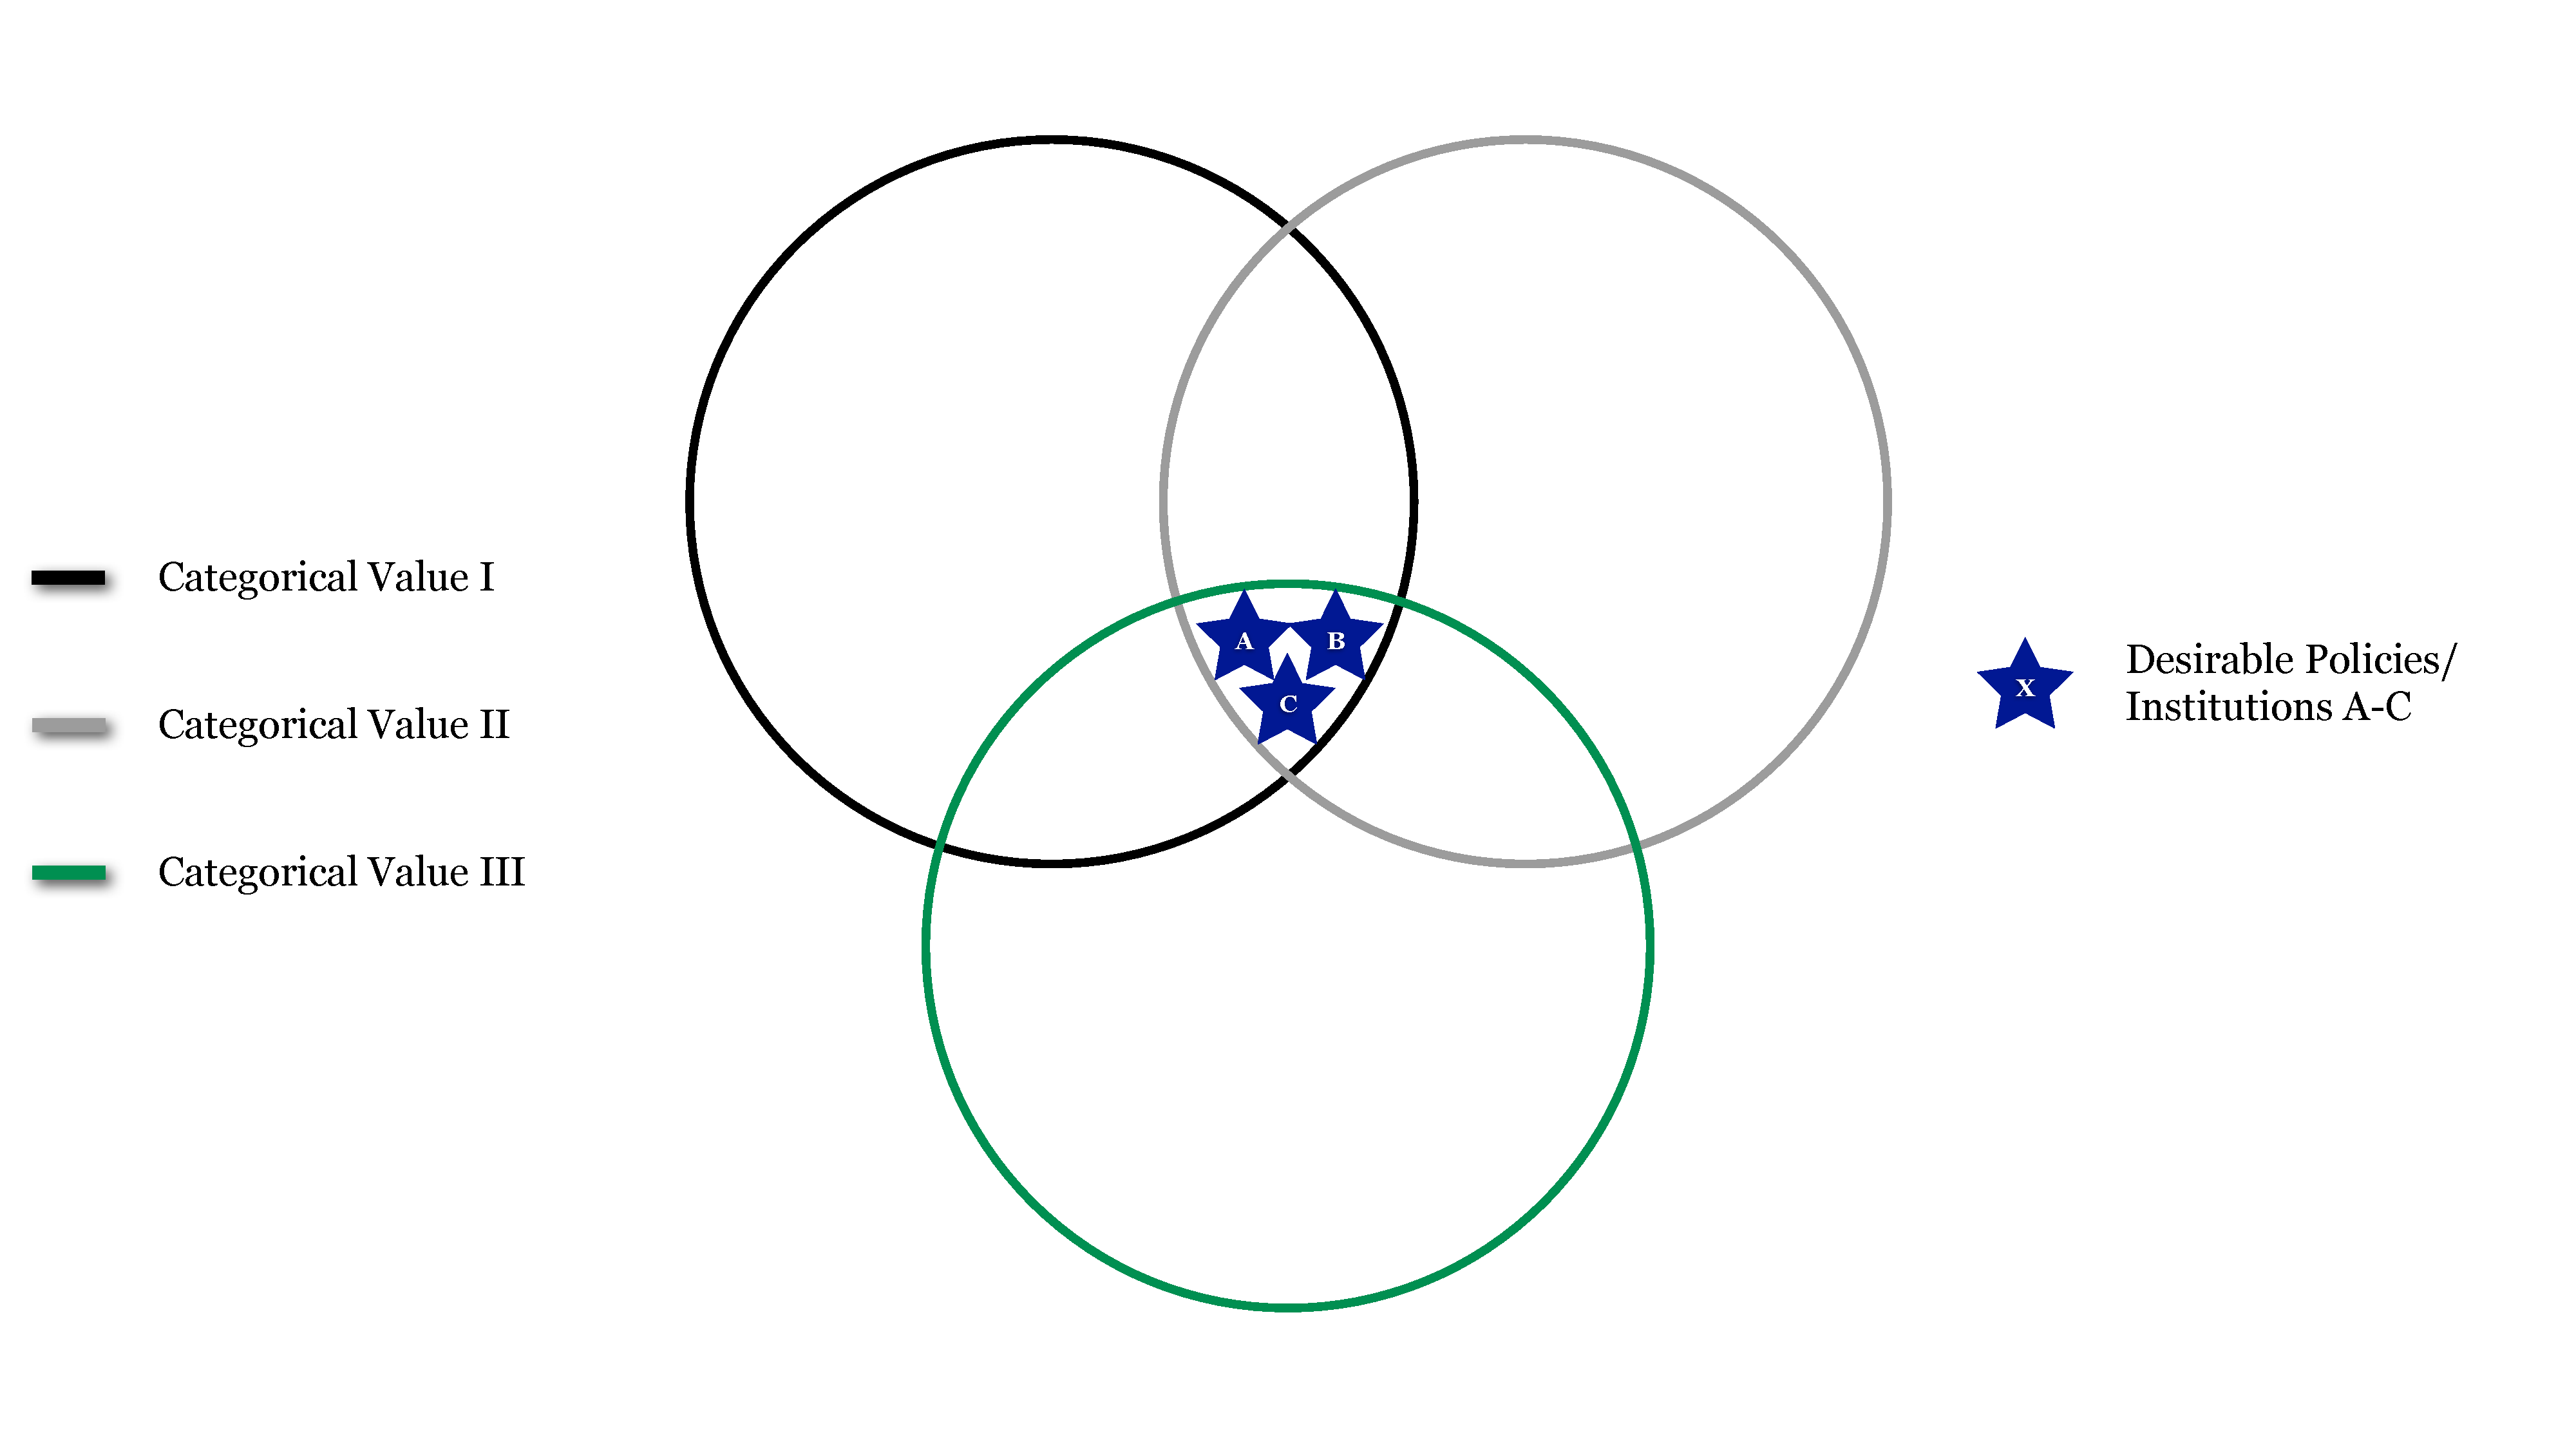
\includegraphics[width=1\textwidth]{euler-values}
			\caption{Euler Diagram of Three Values}
			\label{fig:euler-values}
		\end{figure}

		All remaining values must be reconciled within this intersect of categorical values of liberalism.
		Here too, even supposedly outsized cardinal gains in any of the remaining values cannot be traded off nominal violations of categorical values.
	\item
		In part, I resolve these conflicts by offering trade-offs.
		This works only for values that are continuous in their realization, as may be the case for the tired conflict between equity and efficiency in taxation.
%add href
		I suggest that the trade-offs offered by such conflicting, continuous values depend crucially on the institutional context under which these trade-offs have to be engaged.
		Calling trade-offs, and designing the conditions thereof can be illustrated well in a diagram of \glspl{PPF}, frequently used in economics to illustrate different possible baskets of goods that can be produced by an economy.
		Because paper as this is two-dimensional, \gls{PPF} diagrams frequently only show two goods, but the abstraction carries to any number of $n$ goods in a basket.
		I adapt the traditional \gls{PPF} in \autoref{fig:ppf-values} (p.~\pageref{fig:ppf-values}).
\end{enumerate}

\begin{figure}[htbp]
	\centering
	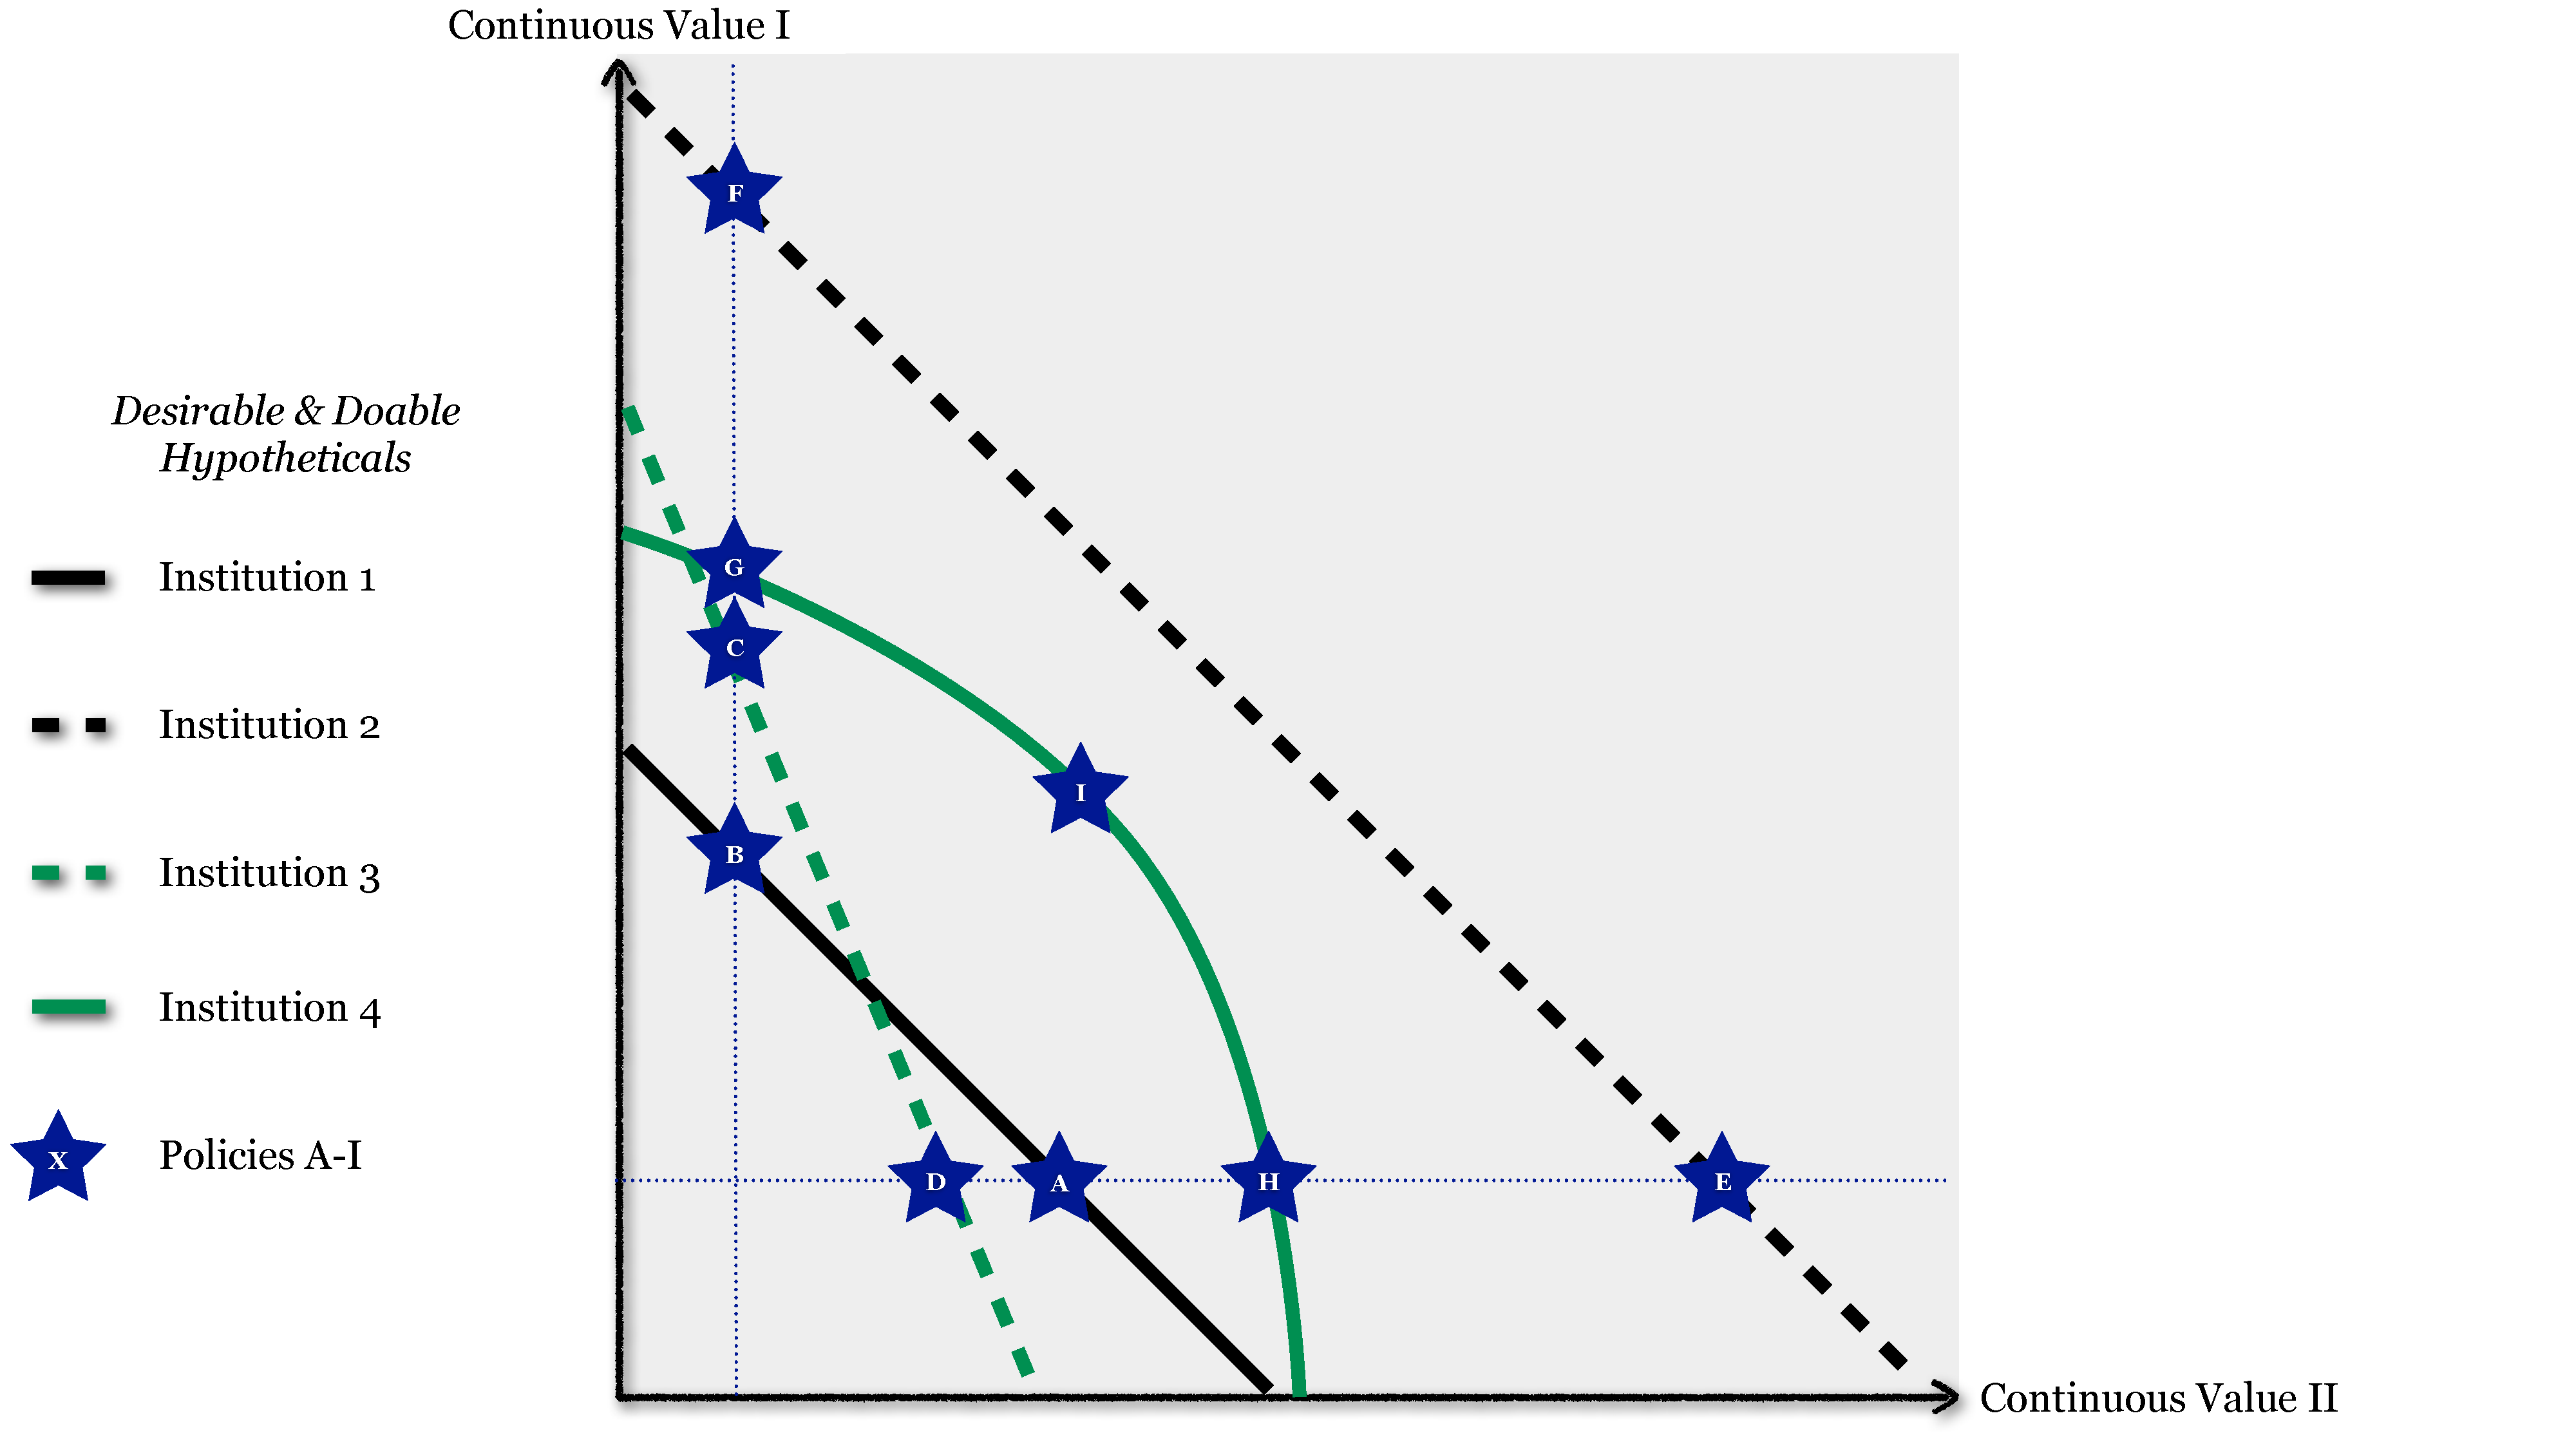
\includegraphics[width=1\textwidth]{ppf-values}
	\caption{Production-Possibility Frontiers of Two Competing Values}
	\label{fig:ppf-values}
\end{figure}%economies of scale variant is still missing

	What are competing goods in a \gls{PPF} diagram are here competing values $I$ and $II$.
	Let us assume for the sake of simplicity that these values can be easily measured and are ratio scaled.
	More of each value is better.
	The four \glspl{PPF} are comprised of those possible combinations of values $I$ and $II$ which are \emph{furthest} from the origin, and thereby strictly preferable over all possible policies \emph{under} the \gls{PPF}.
	As in a static model of the economy, the \glspl{PPF} are exogenously determined by a priori, and posteriori limits of the first order.
	In addition, I argue, these exogenous limits are modified by \emph{institutions} $1$ through $4$.
	 Policies $A$ through $J$ are defined by specific combinations of continuous value $1$ and $2$, along the respective institutions which modify what is logically and empirically possible in this world.

	\autoref{fig:ppf-values} illustrates different policy choices.
	The simplest kind of trade-off is that between two policies along a linear \gls{PPF}, as between $A$ and $B$ on $1$.
	A straight \gls{PPF} implies that the values are substituted at a constant rate:
any increase in $I$ will requires a decrease in $II$ by the same amount.
	The choice between $A$ and $B$, as all other points on $1$ is a zero-sum proposition.
	As we shall see, trade-offs in welfare, taxation and democracy are frequently, if implicitly, presented as such zero-sum choices.
	Alternatives of this sort are inevitable, but they are also normatively less interesting.
	Once values $I$ and $II$ are reduced to the same scale, the choice along the resultant \gls{PPF} becomes trivial or even arbitrary
	\footnote{
		In the technical terms of introductory economics, individual preferences are expressed in \emph{indifference curves}, that is, the lines along those combinations of $I$ and $II$ between which a person is indifferent.
		The intersection between the aggregate of these indifference curves would be the optimal policy point(s).
%is this true?
		If the aggregate indifference curve is curvilinear and reasonably simple, there will be one or few such points.
		If, however, the aggregate indifference curve is \emph{linear} and scaled as the \gls{PPF}, \emph{all} policies along the \gls{PPF} intersect with an identical indifference curve, and there are an infinite number of ideal policy points.
		%I think here's a big question:
%are indifference curves curvilinear or linear? and why? How is this related to scaling?
	}.%add refs to later misunderstandings here

	\gls{PPF} $4$ is curvilinear, and more interesting.
	Here, the rate of substitution varies over different levels of $I$ or $II$.
	For example, around $G$, you have to give up relatively little in $I$ to gain relatively much in $II$.
	The reverse is true around $H$, and substitution is roughly constant around $J$.
	The trade-offs between $I$ and $II$ are non-zero-sum:
you can gain more than you loose.
	Assuming a reasonable aggregate indifference curve (linear or convex), optimal policy will probably lie around $J$.
	As we shall see, concave or other curvilinear \glspl{PPF} abound in welfare, tax and democracy.
	Recognizing the convexity of trade-offs offered by any given institution, or, if possible, moving from lower, linear \gls{PPF} $1$ to a higher, convex \gls{PPF} $4$ will be important to identify desirable hypotheticals.%add later hrefs

	\glspl{PPF} $1$ and $3$ are both linear, but they have different slopes.
	At any level of $I$, compared to \gls{PPF} $1$ you have to sacrifice more in $I$ to increase $II$.
	The moves \emph{along} curve $3$ are otherwise as normatively uninteresting as those along \gls{PPF} $1$ --- the two are just scaled differently --- but the choice \emph{between} these two institutions will be very consequential.
	Compared to institution $1$, institution $3$ will always make it costlier to increase value $II$.
	There are many such consequential choices of institutions in tax, welfare and democracy.
%add hrefs

	\glspl{PPF} $1$ and $2$ both have the same slope, but $2$ is further from the origin.
	By definition, all policies along this higher curve are preferable to all policies on the lower curve --- to everyone
	\footnote{
		Technically, again, \emph{no matter the indifference curve}, the higher, but equally-sloped \gls{PPF} will always be preferable.
	}
	.
	This is the most important of institutional choices to be made.

		%hehe, here's a pretty big part of the story missing:
%the DEMAND side.
%You'd need indifference curves!

%note how justice as fairness falls in-between these \ldots it's somewhere in-between all of those

%why is this pragmatic?

\section[Ontology]{The Ontology of The Doable Hypothetical} \label{sec:ontology}

\textsuperscript{\ref{fn:also-in-europe}}

%ontology is the stuff that I am dealing with

%``(\ldots) every research agenda must start from some basic assumption about human nature, and the assumption of my research agenda is that despite all the evil in the world, at least some humans have, some of the time, a sense of goodness in truly caring for the well-being of others.'' \cite[7]{Steiner2012}

\begin{quote}
	\emph{``But what is government itself, but the greatest of all reflections on human nature?''}\\*
	--- James \citep[143]{Madison1788}
\end{quote}

Doable hypotheticals are preferable to others because, in \citeauthor{Dahl-1989-aa}'s words, ``we must avoid comparing ideal oranges with actual apples'' \citeyearpar[84]{Dahl-1989-aa}.

Deciding just what can, and cannot be done is hard.
If asked as a positive first-order question, the answer is sometimes empirically unclear.
If turned into a second-order question --- as the social sciences are prone to do --- the answer becomes politically contested.
Both extremes do not serve us well:
\begin{enumerate}
	\item
		When all inquiries into the social world are reduced to positive, first-order questions the social sciences effectively abolish themselves and make the status quo epistemologically endogenous, as in:
\emph{social inequality is inevitable human nature, because if it were not, it would not be observed}, or ``the Laws of commerce are the laws of Nature, and therefore the laws of God.'' (\citeauthor{Burke1790} as cited in \citealt[834]{Marx-1867-aa}).%find better source
	\item
	Conversely, when such inquiries assign all positive questions to second-order status, the social sciences hermetically seal themselves off from other disciplines and turn critique into futile, infinite regress, as in:
\emph{``social being [\ldots] determines [\ldots] consciousness''} \citep[Preface]{Marx1859}, including, one might add, Marxist consciousness.
%find out that one piece that argues that social scientists are leftist because they get paid by the state
\end{enumerate}

Instead, the social sciences --- and especially policy analysis --- should find a middle ground, taking on \emph{one second-order question at a time}, while provisionally leaving all other questions to first-order status.

I here ask second-order questions about the welfare state, taxation and democracy and I therefore assume these \emph{institutions} to be malleable.
\emph{Not} under study here are \hyperref[sec:human-nature]{human nature} (p.~\pageref{sec:human-nature}) or the \hyperref[sec:modernity]{modern condition} (p.~\pageref{sec:modernity}), especially of developed states and late capitalist economic production.
I assume these to be constant in the medium run and reasonably approximated in the following sections.

\subsection[Human Nature]{Human Nature} \label{sec:human-nature}
Any second-order prescription for how to organize production, distribution and decision making rests on assumptions about human nature.
For evolutionary anthropology, psychology, behavioral economics and other offspring of now disreputable \citep{Wright1994} sociobiology \citep{Wilson1975} this is a positive first-order question about our prehistoric baggage:
what behavioral, cognitive and emotional dispositions might have been adaptive in the environment of our evolution, and what do we observe today?

\subsubsection[Evolution and Morality]{Evolution and Morality}
Maybe, evolution deserves to be the master ontology of life, and therefore, of human life, too.
Because I sometimes refer to such Neo-Darwinian arguments \citep{Wright1994} and hear them often misunderstood I must reiterate the ontological status of the theory of evolution:

\begin{enumerate}
	\item
		Evolution may dispose us to think, feel and act in certain ways, but does not determine us to do so (\emph{deterministic fallacy}).
	\item
		Evolution yields more (``gradual'' according to Neo-Darwinism) or less (``punctuated'' according \citealt{Elrdredge1972}) stable \emph{equilibria} between environmental conditions and (more or less) adaptive traits of organisms.
		It does not necessarily yield \emph{optimal} configurations, just survival of the relatively fitt\emph{er}.
		Conversely, not all biological features that are observed are necessarily adaptive, but may simply be side consequences of other, adaptive features or developmental vestiges \citep{Gould}.

	Or, in \citeauthor{Bryson2003}'s succinct formulation, ``life wants to be, but it doesn't want to be much'' \citep{Bryson2003}.

	\item \label{itm:nonmoral}
		Evolution is a ``nonmoral'' process \citep{Gould1982}.
		It may tend towards greater complexity and cooperation, including human-like intelligence \citep{Wright2000}, or it may just pursue a random walk, departing from a ``left wall'' \citep[4]{Gould1994} of ``simple beginnings'' \citep[7]{Gould1977}, and inevitably bring some complexity, including \emph{homo sapiens} as a freak outlier \citep{Gould1996}.
		Either way, even if evolution \emph{were} directional, it would not be along any moral dimension intelligible to humans.
This cuts both ways:
		\begin{enumerate}
			\item
				to praise evolutionary results is to fall for a \emph{``naturalistic fallacy''} (\citealt{Moore1903}, as cited in \citealt[K5987]{Wright2000})
			\item
				to criticize them on any moral basis is to commit a \emph{``moralistic fallacy''} \citep{Davis1978}.
		\end{enumerate}
\end{enumerate}

Within these ontological limits, evolution serves me well in this dissertation, because as a materialist, positive and first-order perspective it allows me to limit my second-order inquiries on taxation and democracy.
%include examples!

Unfortunately, evolutionary logic has a way of straying beyond the positive, of encroaching on and negating normative questions, precisely because it purports to explain all life, including human life.
For example, if exclusive fitness were operative in human evolution, does that not, as Social Darwinism suggested, imply that humans \emph{are} unequal, end of story?
More fundamentally --- and less obviously ideological --- if all our flesh, including our brain tissue, evolved in an aimless process, does that not, as overzealous neuroscientists like to test, imply that whichever subjective experiences of consciousness and free will that flesh reports must be wholly illusory, and all questions of morality therefore beside the point?
If we were merely organic, delusional robots, as \citet[Chapter 23]{Wright2000} provocatively asks, what would be wrong with unplugging a few?

This pedestrian thesis is not the place for another mind-body debate, and I am equally awed and outmatched by these and other ``hard problem(s) of consciousness''  \citep{Chalmers1995}.
Still, I must ask the reader to allow me a crude bit of lay metaphysics.

For starters, positive questions on consciousness --- including the downstream issue of free will --- easily run into seemingly obvious logical problems.
If consciousness were positively illusory, who would be left to do the observing?
Conversely, if consciousness were some positive emergent neuronal phenomenon, would not precisely that physical genesis negate subjective experience?
Either way, infinite regress ensues.
Perhaps, as James \citeauthor{Trefil1997} muses, consciousness ``is the only major question in the sciences that we don't even know how to ask'' \citeyearpar[15]{Trefil1997} and maybe, therefore, we need not be bothered, for now.

More fundamentally, whatever we may learn about the (aptly named) ``neural \emph{correlates} of consciousness'' (for example, \citealt{Koch2004}, emphasis added) none of this positive research can, or ever should negate, or infringe on normative questions.
The first-order positive questions of natural science, and the first-order normative questions of the social sciences should be kept neatly apart, because they are \gls{NOMA} \citep{Gould1997}.
Akin to science and religion, first-order positive and normative questions, too are distinct ``domain(s) where one form of teaching holds the appropriate tools for meaningful discourse and resolution'' \citep[3]{Gould2002}:
\begin{quote}
	\emph{``The magisterium of science covers the empirical realm:
	what the Universe is made of (fact) and why does it work in this way (theory).
	The magisterium of religion extends over questions of ultimate meaning and moral value.
	These two magisteria do not overlap, nor do they encompass all inquiry (consider, for example, the magisterium of art and the meaning of beauty).''}
	\\*
	--- Steven Jay \citet[6]{Gould2002} %add first name
\end{quote}

No matter then, how hard-nosed a question we may ask about our evolved nature, these positive inquires must never be mistaken for, or negate normative questions, because these fall into categorically different realms:
\begin{quote}
	\emph{``Our failure to discern a universal good does not record any lack of insight or ingenuity, but merely demonstrates that nature contains no moral messages framed in human terms.
	Morality is a subject for philosophers, theologians, students of the humanities, indeed for all thinking people.
	The answers will not be read passively from nature:
%they do not, and cannot, arise from the data of science.
	The factual state of the world does not teach us how we, with our powers for good and evil, should alter or preserve it in the most ethical manner.''}\\*
	--- Stephen Jay \citet[43]{Gould1982}
\end{quote}

\emph{Ought may imply can} \citep[65]{Kant1794}, but they are still not the same thing.
However much constricted positive science may find us to be, these limits of what we \emph{can} do must never drown out the imperative \emph{ought}.
Perhaps, tautologically, to be human and not another animal, is to arrogantly insist that, in spite of the limited and banal flesh we are made off, we \emph{ought} to be conscious, we \emph{ought} to have free will and we \emph{ought} to say ``ought''.

Maybe, this is the this-wordly obedience to Jesus Christ that Dietrich Bonhoeffer meant --- and died for --- when, faced with fascism he chose ``costly discipleship'' \citep{Bonhoeffer1937}:
``Only he who shouts for the jews is permitted to sing Gregorian chants'' (Bonhoeffer 1933 as cited and translated in \citealt[35]{DeGruchy1999}).
Fascism, after all, was the modern ideology to radically negate any ``ought'' for whichever group (``race''!) was supposedly biologically superior, and de-facto militarily stronger.
Perhaps, such rejection of ``ought'', too, makes the ``banality of evil'' that Hannah \cite{Arendt1963} recognized in an Adolf Eichmann on the stand in Jerusalem.
Eichmann, after all, might ``excuse[\ldots] himself on the ground that he acted not as a man but as a mere functionary [\ldots] since after all, someone had to do it'' \citep[K286f.]{Arendt1963}.
Such \emph{acts of state} defy \emph{ought}, because, to an ``unthinking'' Eichmann \citep[K187f.]{Arendt1963}, history --- as evolution --- just \emph{is}.

Such lay metaphysics might be crude, but they are \emph{not} entirely beside the point of welfare, taxation and democracy.
As I argue later, a milder, but similar conflation of \emph{can} and \emph{ought}, of second-order positive, and first- and second-order normative questions plagues some social science, especially when it \hyperref[chap:hypotheticals-matter]{lacks hypotheticals} (\autoref{chap:hypotheticals-matter}, p.~\pageref{chap:hypotheticals-matter}).
In the social sciences, too, the line between an emerged, evolved, ``grown order'' and a ``made order'' is sometimes blurred, negating political \emph{oughts} --- and not always as elegantly and explicitly as by \cite[37]{Hayek1973}.

\subsubsection{Evolution and Institutions}
We need not confine evolutionary explanations to our biology alone, or, conversely, reduce all behavior, cognition and emotion to some strictly physical (genetic) reason.
Instead, we can apply evolutionary explanations to \emph{culture} and \emph{institutions}, too.

In fact, the tired --- and often unproductive --- nature vs.\ nurture controversy is moot:
we are neither blank slate
\footnote{
	\ldots \emph{aka.} \emph{tabula rasa} or \emph{homo sociologicus}, as \cite{Dahrendorf1965} quipped.
}
for behaviorism to condition or society to write on, nor a physically determined animal, but essentially \emph{both} nature and nurture.
Our bodies and culture-ready brains genetically \emph{co-evolved} with co-adaptive memes \citep{Dawkins1976} to make us the ``hypercultural species'' that we are \citep[K175]{Henrich2007}.
Relatively ill-equipped in instincts, we need to \emph{learn} (or \emph{imitate}) what to eat and hunt --- and how to build a blast furnace.
Perplexingly, it is in our \emph{nature} to rely on \emph{culture}:
as our brain allowed us to learn easily, our culture developed cooking, and our digestive tract adapted to broken-down proteins, as illustrated in \autoref{fig:coevolution-nature-culture} (p.~\pageref{fig:coevolution-nature-culture}, \citealt[confer][]{Henrich2007}).

\begin{figure}[htbp]
	\begin{center}
	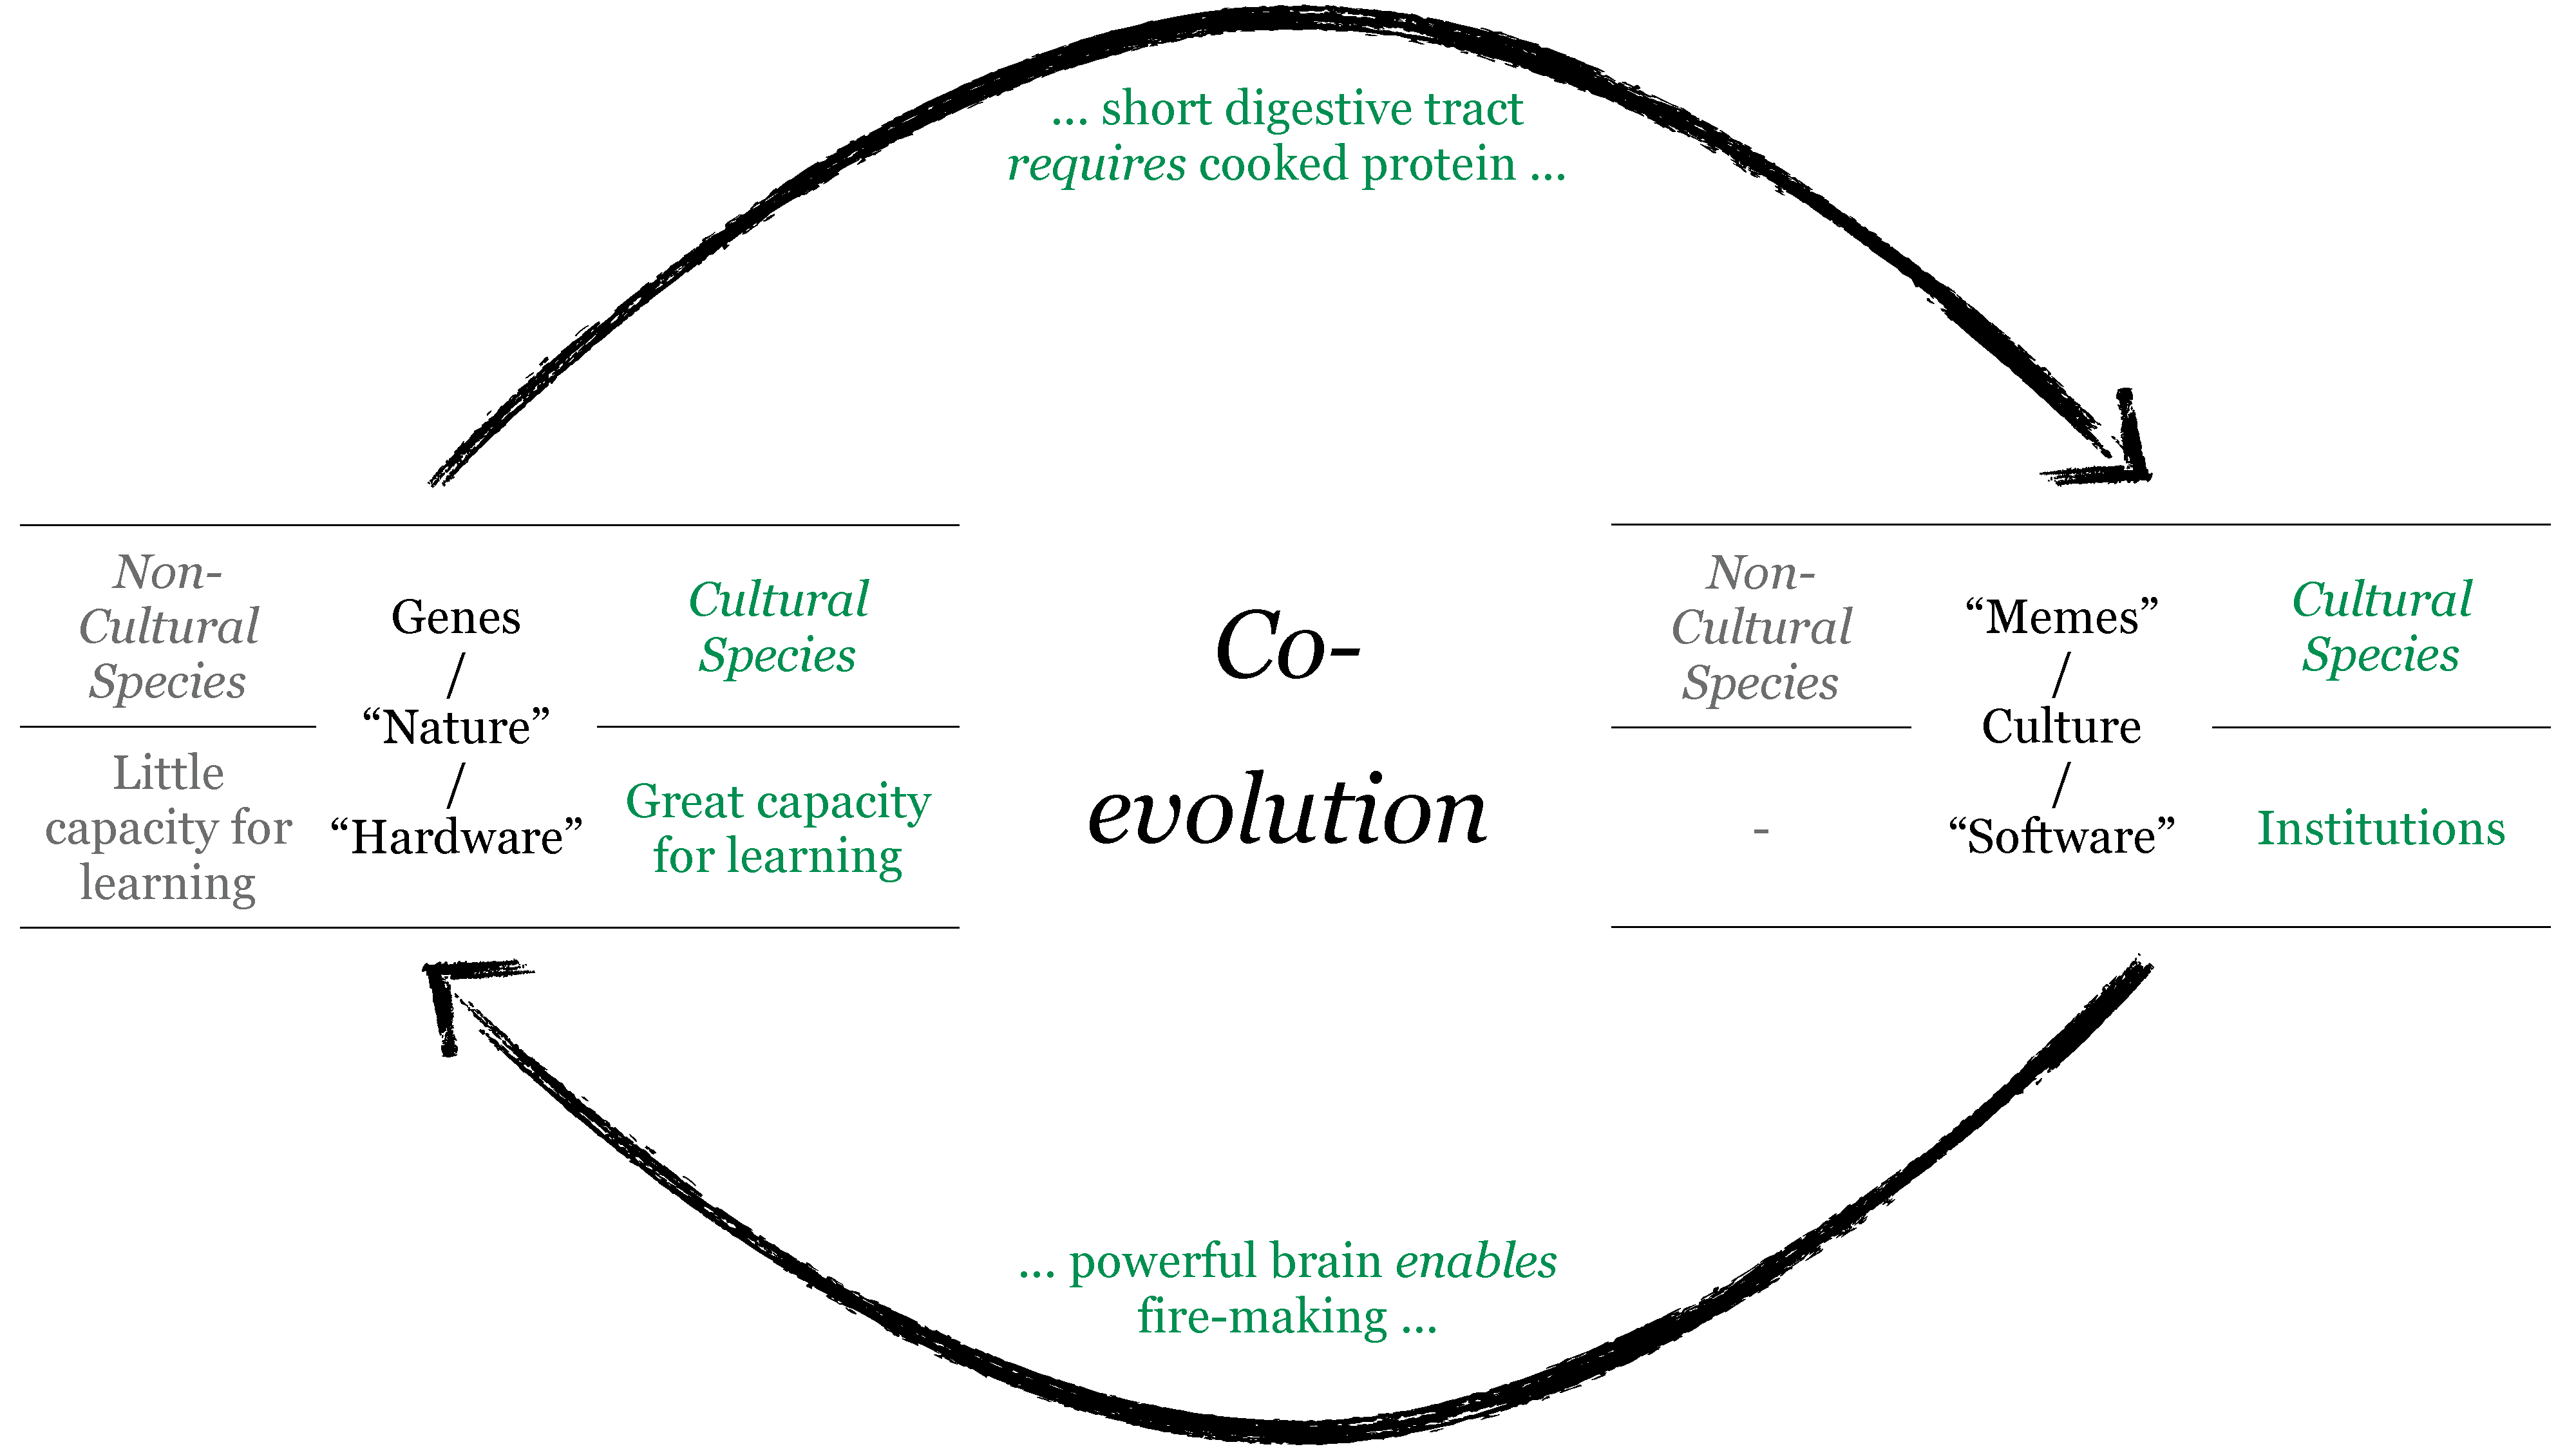
\includegraphics[width=1\textwidth]{coevolution-nature-culture}
	\caption[Coevolution of Nature and Culture]{The coevolution of nature and culture, with some examples}
	\end{center}
	\scriptsize{Own illustration, based on \citet[K120ff]{Henrich2007}}
	\label{fig:coevolution-nature-culture}
\end{figure}

This is the evolutionary blockbuster of humans:
we moved the locus of our evolutionary adaptation from genes to memes \citep{Dawkins1976}.
Instead of ``hard-coding'' all adaptive traits, we learn (or imitate) the more complex and more malleable software of culture (\citealt{Boyd1985}, \citealt[K196ff]{Henrich2007}), written not in \gls{DNA}, but coagulated into institutions.

Paradoxically, as the naturally hypercultural species, we might gain some leeway from our biology, but simultaneously loose it to culture, because evolved culture too, must be (co-)adaptive to our biology, environment and, crucially, our \emph{past}, path dependent culture (\emph{evolutionary anthropology}, for example, \citealt{Wright2000}).
As sociologists like to say about institutions --- the coagulates of culture --- culture, too, may \emph{enable us as it constrains us} \citep[for example,][3]{Hodgson2006}.

Here lurks another positive first-order dead end:
if present culture is, by definition, sufficiently (co-)adaptive to persist, does that not imply that any new, improved culture could and \emph{would} emerge by said evolutionary process if, \emph{and only if}, it were (co-)adaptive to our nature and environment and sufficiently incremental from past culture?
If, therefore, culture and institutions, too, were strictly positive phenomena unamenable to human will, would the social sciences and political critique not be completely beside the point? %cite Neiman somewhere in here? for example, http://www.fortschrittsforum.de/debattieren/bildung-modernisierung/artikel/article/bequemlichkeit-ist-was-fuer-realisten.html#tx-comments-comments-163

Hardly so.
Here, as in all evolutionary arguments, the \emph{can} need not, and must not eclipse the \emph{ought}.
We may not be able to make arbitrary institutions, but, axiomatically, we \emph{can} build \emph{progressive} institutions:
they help us achieve normative ends, by first responding to our evolved cultural and natural dispositions, then transcending them.
At least since Enlightenment dawned, we get to make our own history (a little), and build or break (some) institutions as an act of will --- that is \hyperref[itm:pragmatic-ethics]{ethical pragmatism} (p.~\pageref{itm:pragmatic-ethics}).

To build institutions is to emancipate ourselves from the meaningless process that bore us as expendable containers of ``selfish genes'' \citep{Dawkins1976} and to heed that call for morality, that we among the earth's animals may hear clearest, because through institutions, we \emph{can} turn reflexive on our innate behavior, cognition and emotions.

\subsection[Modernity]{The Modern Condition} \label{sec:modernity}
Maybe this is as good a definition of modernity as any:
the project by which we reflect on what might be innate to our existence and inevitable about our physical world, and deliberately build institutions accordingly.
Thus advises a machiavellian \citeyearpar{Machiavelli1532} \citeauthor{Mandeville1714} to turn ``private vices by dextrous management of a skillful politician (\ldots) into public benefits'' \citeyearpar[213]{Mandeville1714}, thus threatens a somber \cite{Hobbes-1651-aa} our inner wolves with an even more powerful metaphorical beast, and thus asks us a moralizing \cite{Smith-1776-lq} to receive from others ``from their regard to their own interest'' --- or any number of other ``idea[s] of the world as open to transformation, by human intervention'' \citep[94]{Giddens1998}.

Modernity, as evolution, is often misused or misunderstood, and so again, I must briefly clarify its ontological status for my purposes:

\begin{enumerate}
	\item
		The modern project need not be confined to a specific location or era, nor need it be one-directional or linear, but it might arise in different places at different times, it might wax and wane, explode and collapse.
		While Europe and North America in the early 21st century may constitute high points in this project, the modern project is not wedded to any specific historical context or even the institutions which it bore, but rather, modernity is a \emph{cultural} and \emph{cognitive} phenomenon \citep[26, emphasis added]{JonesJones-2003-aa}.
	%include reference to diamond on the arbitrariness of why modernity happened in western europe
	\item
		The modern project need not be inherently good nor necessarily lead to desirable outcomes:
modernity may well bear alienation \citep{Adorno1966}, or even lead to catastrophe \citep{Bauman1989} and not all of its (ongoing) advances may yield progress.

		However, the inverse is true:
to think progress implies a modern mindset, and to get it done requires modern institutions.

	\item
		It should be redundant to say that my dissertation ontologically assumes a modern condition, because tautologically, sociology is about finding answers to the questions modernity raises \citep[325]{Harriss2000}, and ``postmodern sociology [therefore] an impossibility'' \citep[169]{Miles-2001-aa}.

	And yet, ``modernity'' seems to be a concept fallen out of fashion, superseded by (occasionally loose) talk of various post-isms (for example, \citealt{Lyotard1984}, Baudrillard) or second and reflexive modernities \citep[for example,][]{BeckBonss-2003-aa}.

	Whatever the value of these and other contributions, in welfare, taxation and democracy I find no contradictions that would require such categorical labels or the nascent theories they stand for.
	In fact, I suspect that a thoroughly \emph{modern} analysis of welfare, taxation and democracy may resolve many of those contradictions which reflexive modernity prematurely identifies, and clarify some of the uncertainties in which postmodernity revels.
	For instance, maybe, equipped with a rational and deep understanding of the mixed economy and externalities, we find that ``de-nationalization'' \citep{BeckGrande-2007-aa} and ``risk society'' \cite{Beck-1992-aa} are neither inevitable, nor particularly descriptive but simply avoidable and unsurprising cooperation problems, instead.
%add \href

	I here reflect on many dysfunctions of the presently observed, undoubtedly modern institutions of welfare, taxation and democracy, but I need not get ``all meta'' about modernity, because precisely such ``reflexivity is a modern, not postmodern set of attitudes and practices and that ritualized postmodern caviling against modernity is ahistorical and inaccurate, not to mention dispiriting'' \citep[1119]{Sica-1997-aa}.

	Also, as I promised earlier, this \emph{is} a pedestrian thesis.
\end{enumerate}

What then, are these indispensable modern institutions that I here assume as ontological entities, that which defines the ``doable''?

\subsubsection{States and Markets}
For the production and distribution of goods, they are state plan (but not \emph{nation state}) and market exchange (but not any particular x-\emph{capitalism}).
For collective decision making, they are a state equipped with an effective monopoly on the use of force and devoted to some popular participation \citep[compare][96]{Giddens1998}.

These two, states and markets, both \emph{brought} and \emph{constitute} the modern condition:
they hyper-charged functional differentiation \citep{Smith-1776-lq} to reach near-planetary breadth (for example, international trade, citizenship) and near-universal depth (for example, commodification, family law), they altered or replaced much of the evolved culture (for example, kin) and institutions (for example, tribe) adaptively fit only at smaller scale \citep{Diamond1997}, replaced such mechanical by organic solidarity \citep{Durkheim-1893-aa} and bore a social world that is complexly interacting \citep[for example,][]{Merton-1968-aa,Merton-1936-aa}.

These two are also the meta-institutions that both define and allow welfare, taxation and democracy.
Welfare and taxation exist only, as I explain later, in mixed economies of both market exchange and state plan.
Taxation and democracy alike, to become real, must be enforced by a state with an effective monopoly on the use of force.%add \href

As all modern institutions, state and market are based on a particular model of human nature, in this case, a
\begin{enumerate}
	\item rational and %also included in the axioms
	\item individual
	\item utility-maximizing %also included in the axioms
\end{enumerate}
\emph{homo economicus} \citep[maybe first in][]{Mill1848}.
The state gets an amoral, but opportunistic \emph{homini lupus} to behave by threatening monopolistic force \citep[as in][]{Hobbes-1651-aa}.
The market, in turn, lures a self-seeking, but rational ``butcher, [\ldots] brewer, or [\ldots] baker'' into providing ``our dinner'' --- and all else --- ``from their regard to their own interest'' \citep{Smith-1776-lq}.

\subsubsection[Nonzero]{Non-Zero-Sumness \label{sec:nonzero}}
But, as other modern institutions, state and market not only assume this human nature, they also allow homo economicus to transcend her own limits.
As \emph{individual} utility-maximizers, she runs into problems whenever her supposed selfishness prevents otherwise mutually advantageous interactions.
This rough typology specifies the class of games which homo economicus is ill-equipped to solve:

\begin{enumerate}
	\item
		\emph{Zero-sum} games display constant sums of payoffs over all cells, or possible interactions.
		One player's gains equal another player's losses:
the cake does not grow, but is only sliced up differently.
		By definition, a zero-sum game is pareto optimal:
no one can be made better off, without making someone else worse off
		\footnote{
			Critics of economic growth (but not \gls{GDP}!) should carefully ponder the implications of such a scenario:
a world with no economic growth is a world where \emph{all} human interactions are zero-sum.
			Empirical literature on, for example, rentier economies, have chronicled the corrupting influence that zero-sumness may have on a political process, when all decisions create \emph{nothing but} winners and losers \citep{Beblawi1990}.
		}.

		Terms of trade, the ratio of units of goods that a country has to export for any unit of imports, is an oft-cited (rare) example of zero-sumness in advanced economies.%add citation

		A trivial example of zero-sumness, theft, (without spillovers) is illustrated in \autoref{tab:theft}:
all cells yield the same $\sum{\text{payoffs}}=2$.

	\item
		\emph{Non-zero-sum} games have different sums of payoffs, or possible interactions.
		One players gains are not equal to another players losses:
the cake can grow or shrink.
Positive-sum games are equivalent to negative-sum games, because the absence of a loss (a negative-sum outcome) is a gain (a positive-sum outcome).
		For the sake of simplicity, I often refer to only gains or positive-sum outcomes, but mean all non-zero-sum games.
		Crucially, non-zero-sumness does not imply that gains are shared equally, or at all.
Non-zero-sum games need not even imply (weak) pareto-improvements, if one players looses less than another gains in a Kaldor-Hicks-improvement \citep{Kaldor1939,Hicks1939}.

	Non-zero-sum games further break down into:
	\begin{enumerate}
		\item
			\emph{Games of total harmony} are situations in which self-interested players will \citeauthor{Nash1951}-equilibrate at an interaction that reaps all non-zero-sumness
			\footnote{
				\emph{Strategies}, or players' moves, form a \emph{Nash equilibrium} if they are mutually \emph{best responses}.
				Best responses, in turn, are the utility-maximizing move for a player, \emph{given} the other player's choice.
\emph{Dominant strategies} are those best responses that maximize payoffs over \emph{all} choices of the other player(s).
				The \emph{social welfare optimum} is realized under those combinations of strategies that maximize the aggregate payoffs of all players.
				\cite{Kleinberg-2009-oz} provide a great introduction into game theory and its basic concepts.
			}.
			By definition, a game of total harmony offers pareto improvements:
at least one player \emph{can} be made better off, (at least) without making someone else worse off.

			Under some assumptions, opening up to free trade famously is such a game of total harmony \citep{Ricardo1817}.
			It is roughly illustrated in \autoref{tab:trade}:
at $\sum{\text{payoffs}}=6$, the north-western cell yields the highest, social optimum and it is also the only (!) set of mutually best responses, and thereby, the unique Nash equilibrium.
			In short:
trade and other games of perfect harmony should take care of themselves.

		\item
			\emph{Cooperation problems} plague non-zero-sum situations where the social welfare optimum is not also (at least) \emph{a} Nash equilibrium.
			Here, at least one player may gain more than all others stand to loose.
%is this true?
			Such games cannot be Pareto-, but only Kaldor-Hicks improved.

			The canonical example of a cooperation problem, a \gls{PD}, is given in \autoref{tab:PD}:
here the socially optimal (smallest) payoff $\sum{\text{payoffs}}=2$ prison years its in the north-western cell, but it does not constitute a mutually best response.
			In fact, no matter what the other player does, one is always better off betraying:
the south-eastern cell is not only a mutually best response and thereby the Nash equilibrium, but even a mutually \emph{dominant} strategy at a dismal aggregate prison sentence of $\sum{\text{payoffs}}=6$ years.

			The \gls{PD} and related cooperation problems can model many of the economic and political challenges facing us today, including global warming \citep[for example,][]{Stern-2006-aa} and herding in financial markets (from \citealt {Keynes1936} to \citealt{Banerjee-1992-aa}).
			I also identify \gls{PD}-style problems in welfare, taxation and democracy.
%add \hrefs
	\end{enumerate}
\end{enumerate}

\begin{table}
	\caption[The Theft Game]{Theft as a Zero-Sum Game}
	\label{tab:theft}
	\begin{center}
	\begin{tabular}
		{m{1cm}
		m{2,3cm}
		m{2,3cm}
		m{2,3cm}
		m{2,3cm}}


 %empty cell
& %empty cell
& \multicolumn{2}{c}{\emph{Player A}}
\\


 %empty cell
& %empty cell
&Does not steal
&Steals
\\

\cline{3-4}

\multicolumn{1}{c}{\multirow{4}{*}{\emph{Player B}}}
& \multirow{2}{2,3cm}{Does not steal}
& 	\multicolumn{1}{|r|}{1}
& \multicolumn{1}{r|}{2}
\\


\multicolumn{1}{c}{}
& \multicolumn{1}{c}{}
& \multicolumn{1}{|l|}{1}
& \multicolumn{1}{l|}{0}
\\

\cline{3-4}

\multicolumn{1}{c}{}
& \multirow{2}{2,3cm}{Steals}
& \multicolumn{1}{|r|}{0}
& \multicolumn{1}{r|}{1}
\\


\multicolumn{1}{c}{}
& \multicolumn{1}{c}{}
& \multicolumn{1}{|l|}{2}
& \multicolumn{1}{l|}{1}
\\

\cline{3-4}

\end{tabular}
\end{center}

	\scriptsize{
		Player A and Player B both have a good.
		They can steal from each other, or not steal.
		By heroic assumption, theft has no interaction costs and does not erode trust or security.

		Payoffs are units of enjoyment of goods.
		Higher is better.
		As always, cardinal numbers are examples, only ordinal relations matter.}
\end{table}


\begin{table}
	\caption[The Trade Game]{Ricardian Trade as a Game of Perfect Harmony}
	\label{tab:trade}
	\begin{center}
	\begin{tabular}
		{m{1cm}
		m{2,3cm}
		m{2,3cm}
		m{2,3cm}
		m{2,3cm}}

%empty cell
&
& \multicolumn{2}{c}{\emph{Home}}
\\


%empty cell
&
&Trade
&Autarky
\\

\cline{3-4}

\multicolumn{1}{c}{\multirow{4}{*}{\emph{Rest of the World}}}
& \multirow{2}{2,3cm}{Trade}
& 		\multicolumn{1}{|r|}{2}
& \multicolumn{1}{r|}{1}
\\


\multicolumn{1}{c}{}
& \multicolumn{1}{c}{}
& \multicolumn{1}{|l|}{4}
& \multicolumn{1}{l|}{3}
\\

\cline{3-4}

\multicolumn{1}{c}{}
& \multirow{2}{2,3cm}{Autarky}
& \multicolumn{1}{|r|}{1}
& \multicolumn{1}{r|}{1}
\\


\multicolumn{1}{c}{}
& \multicolumn{1}{c}{}
& \multicolumn{1}{|l|}{1}
& \multicolumn{1}{l|}{1}
\\

\cline{3-4}
\end{tabular}
\end{center}

\scriptsize{
	Home country and Rest of the World can decide to open up to trade or remain under autarky.
	Because both countries have different opportunity costs, as per \citeauthor{Ricardo1817}'s theorem of comparative advantage, they both stand to gain from trade, if possibly unequally.

	Payoffs are the baskets of goods to be consumed.
	Higher is better.
	As always, cardinal numbers are examples, only ordinal relations matter.

	Trade cannot be adequately modeled in two-dimensional payoff-matrix with only two players because, trivially, if one player reverts to autarky, the other player must also choose autarky because there is no trading partner left.
	I ignore that problem here by assuming that the rest of the world will always find some exogenous trading partner.
}
\end{table}

\begin{table}
	\caption[The Prisoners' Dilemma Game]{The Prisoners' Dilemma as a Cooperation Problem}
	\label{tab:PD}
	\begin{center}
	\begin{tabular}
		{m{1cm}
		m{2,3cm}
		m{2,3cm}
		m{2,3cm}
		m{2,3cm}}

%empty cell
&
& \multicolumn{2}{c}{\emph{Prisoner A}}
\\


%empty cell
&
&Stays Silent
& Betrays
\\

\cline{3-4}

\multicolumn{1}{c}{\multirow{4}{*}{\emph{Prisoner B}}}
& \multirow{2}{2,3cm}{Stays Silent}
& 	\multicolumn{1}{|r|}{1}
& \multicolumn{1}{r|}{0}
\\


\multicolumn{1}{c}{}
& \multicolumn{1}{c}{}
& \multicolumn{1}{|l|}{1}
& \multicolumn{1}{l|}{2}
\\

\cline{3-4}

\multicolumn{1}{c}{}
& \multirow{2}{2,3cm}{Betrays}
& \multicolumn{1}{|r|}{2}
& \multicolumn{1}{r|}{3}
\\


\multicolumn{1}{c}{}
& \multicolumn{1}{c}{}
& \multicolumn{1}{|l|}{0}
& \multicolumn{1}{l|}{3}
\\

\cline{3-4}
\end{tabular}
\end{center}
\scriptsize{
	Prisoner A and Prisoner B are both arrested, but police has insufficient information for a conviction.
	The two are separated, and police offers both independently the same leniency deal:
if one betrays the other, she will go free, and the other prisoner goes to jail for 2 years.
	If both betray one another, they will both go to jail for 3 years.
If they both stay silent, they will only be charged with a minor crime and get 1 year in jail.

	Payoffs are years in jail.
	Lower is better.
	As always, cardinal numbers are examples, only ordinal relations matter.}
\end{table}

If we are to reap the (great) benefits of non-zero-sumness, homo economicus must be able to successfully play these classes of games.
She should do well in games of perfect harmony that cater to her selfish utility maximization, but might flounder cooperation problems.
As a maximizer of \emph{individual} utility, she cannot see the bigger picture of aggregate welfare.

Such is, for example, the logic of a \citeauthor{Hobbes-1651-aa}ian war of everyone against everyone:
all would be better off if they ceased fighting, but in a world where everyone is armed and angry, any individual homo economicus better not be a pacifist.
In fact, security may be modeled as a \gls{PD}, as in \autoref{tab:PD-security}.

\begin{table}
	\caption{Security as a Prisoners' Dilemma}
	\label{tab:PD-security}
	\begin{center}
	\begin{tabular}
		{m{1cm}
		m{2,3cm}
		m{2,3cm}
		m{2,3cm}
		m{2,3cm}}

%empty cell
&
& \multicolumn{2}{c}{\emph{Homo homini \ldots}}
\\


%empty cell
&
&\ldots ovis
& \ldots lupus
\\\\ %why more slashes?

\cline{3-4}


\multicolumn{1}{c}{\multirow{4}{*}{\emph{Homo homini \ldots}}}
& \multirow{2}{2,3cm}{\ldots ovis}
& 	\multicolumn{1}{|r|}{2}
& \multicolumn{1}{r|}{3}
\\


\multicolumn{1}{c}{}
& \multicolumn{1}{c}{}
& \multicolumn{1}{|l|}{2}
& \multicolumn{1}{l|}{0}
\\

\cline{3-4}

\multicolumn{1}{c}{}
& \multirow{2}{2,3cm}{\ldots lupus}
& \multicolumn{1}{|r|}{0}
& \multicolumn{1}{r|}{1}
\\


\multicolumn{1}{c}{}
& \multicolumn{1}{c}{}
& \multicolumn{1}{|l|}{3}
& \multicolumn{1}{l|}{1}
\\

\cline{3-4}
\end{tabular}
\end{center}
\scriptsize{
	Two homo sapiens are both living in a \citeauthor{Hobbes-1651-aa}ian primordial state of war.
	They can either be peaceful \emph{obis} (latin:\ sheep), or violent \emph{lupus} (latin:\ wolves) to their fellow men.
	To be violent is costly, but promises a meal of sheep-like humans, or at least their resources (food, shelter).
	If you are eaten, or, more benignly, robbed of food and shelter as a peaceful sheep, you receive no payoff, because either way, you must die or starve.
	If two wolves meet, both engage in costly violence but receive no extra resources.

	Payoffs are utility, as in food or shelter.
	Higher is better.
	As always, cardinal numbers are examples, only ordinal relations matter.}
\end{table}

In a more realistic model with many players instead of just two, the cooperation problem may only exacerbate.
If you were the only wolf amongst many sheep, violence may be especially cheap, because your potential victims are plenty and helpless.
Conversely, being a lone sheep amongst many wolves will be especially risky for the sheep, and costly for the wolves who need to be competitively violent.
At such a larger scale, the \gls{PD} of security evolves into an arms race with ever costlier, but fruitless violence:
the original tragedy of the commons \citep{Hardin-1968-aa}.

Naturally ``stuck in-between'' \citep{Lehrer2012} the selfishness of homo economicus and our capacity for altruism
\footnote{
	Altruistic behavior, according to \cite{Wilson2012} and before him \cite{Darwin1859}, is an emergent property of the \emph{group}, following group selection.
	According to mainstream sociobiology \citep[and initially][]{Wilson1975}, altruism emerges at the \emph{individual} level by a strategy of inclusive fitness or genetic nepotism, helping others as they are related.
},
as ever the ``hypercultural species'' \citep[K175]{Henrich2007}, cooperative exploitation of non-zero-sumness, as much else, does not come to us robotically, or by instinct as it does to the eusocial insects \citep{Wilson2012}.
In humans, such cooperation is \emph{contingent} on culture or institutions.

\subsubsection{The Genesis of Cooperation}
Luckily for us, history listened to \citeauthor{Hobbes-1651-aa} and brought such an institution for large-scale cooperation, when it bore those powerful \emph{Leviathans}, whom we have since successfully trained into rule-of-law, and even democratic states.

Two theories of the genesis of states are instructive here:
\begin{enumerate}
	\item
		Maybe, states are simply the largest remaining of pre-historic, atomistic racketeers who threatened \emph{with} well as \emph{protected from} violence \citep[182]{Tilly-1985-aa}.
		These initially small-scale racketeers morphed into proto-states and then states as new technology, and --- equivalently --- economies of scale allowed them to produce and distribute violence at a larger scale, for lower cost \citep{Tilly-1985-aa}.
	\item
		Or maybe, (nation!) states grew out of kinship ties and our capacity for genetic nepotism \citep{Hamilton1964,Axelrod1981a}, as the initially real blood lines became ever thinner and eventually illusory and fake, yet effective \citep{Van-den-Berghe-1981-aa,Gellner-1983-aa}.
\end{enumerate}

The two stories need not be mutually exclusive, but may instead complement one another.
After all, \citeauthor{Tilly-1985-aa}'s materialist account of state genesis does not so much explain away the cooperation problem, but reverts it to the level of individual thugs who make up the racketeering mafia.
As Coppola's ``Godfather'' (1972, 1974, 1990) trilogy illustrates, even in the 20th century, successful organized crime is not easy, and hinges on trust.
Anecdotally, in the case of the Corleone organization, cooperation is built on family ties, alluding to theories of inclusive fitness as nepotism.
Maybe, economies of scale and first genetic, later imagined nepotism \emph{both} drove state making, only at different levels.
%note that this matters for the later argument on property! Take this up somewhere!

Against this backdrop, the development of governance in the modern era, including sequentially security, the rule of law, democracy and welfare \citep[compare][]{Marshall-1950-aa} is a project of \emph{both} consolidating, and steering a powerful but dangerous monopoly on violence or illusion of kinship, respectively.
Absent such training, states are quite scary beasts, as \citeauthor{Hobbes-1651-aa}'s frontispiece of \emph{The Leviathan} illustrates.
Both theories of their genesis imply a slippery slope.
Supercharged by economies of scale in the production of violence, those monopoly producers of violence may tend towards parasitic government.
``Imagined communities'' \citep{Anderson-1983-aa}, in turn, enabling cooperation by increasingly fabricated nepotistic sentiment, may always risk turning exclusive, or even fascist if the quasi-biological notions run loose.

Here again, the modern age has borne deliberate (meta?-)meta-institutions to govern an evolved structure, including constitutions, rule of law and democracy.
However, all these modern additions to statehood should not distract from its defining innovation:
an effective monopoly on the use of force, without which we are back to a very, very dismal square one.
``You cannot get to Jefferson and Madison without going through Thomas Hobbes'' --- in Iraq \citep{Diamond-2004-aa}, or elsewhere.
%page number missing

Modern markets, and the intricate games of perfect harmony they provide for homo economicus to solve and thrive, too, depend on this monopoly of force.
From property rights, to contract law and fiat money, commerce always rests on effective enforcement:
to enter any such deals in the first place, you must believe that really, \emph{pacta sunt servanda}, that promises \emph{will} be kept --- or made to be kept, anyway.

It is, in fact, this shadow of violence that enables markets in the first place, that allows us to \emph{transform} cooperation problems into games of perfect harmony, and thereby, to \emph{solve} them.

States and markets are, the atomistic reading of \citeauthor{Hobbes-1651-aa} and \citeauthor{Smith-1776-lq} aside, a feat of great cooperation.
Almost magically, they freed us off that \citeauthor{Malthus1798}ian curse, by which our geometric population growth must always outstrip our \emph{arithmetric} economic growth, and starve us
\footnote{
	\cite{Malthus1798} might have been correct only about some periods of human history, and anyway, was anachronistic in his time, when functional differentiation was already well under way.
}.
The modern escape from that iron law of population (or resources, or carbon, and so on) \emph{was}, \emph{is} and \emph{will} be to make economic growth above-linear, too:
to reap non-zero-sumness, to functionally differentiate and to harvest economies of scale.
If at different altitudes of abstraction, these all imply the same prescription:
cooperation \emph{is} our one ticket out of hardship and subsistence (a notion to which I return in the \hyperref[sec:growth-solidarity]{later} in \autoref{sec:growth-solidarity}, p.~\pageref{sec:growth-solidarity}).

\subsection{Contingent Homo Economicus} \label{sec:contingent-homo-economicus}
To think about welfare, taxation and democracy, then, homo economicus is both inescapable and inadequate.

\subsubsection{Inescapable Homo Economicus}
As an ontological model, homo economicus is inescapable, because it comes part and parcel with the meta-institutions of state and markets.
To think of coercive power or supply and demand is to invoke an individual utility-maximizer.
By extension, to ponder welfare, taxation and democracy, too, implies this view of human nature, for if we were neither \emph{individual} nor \emph{utility maximizers}, altruism, allocation and decision making would come to us automatically.
Alas, it does not.

\paragraph{Materially Possible.}
Moreover, market and state, along with their view of human nature are good ontologies for a second-order inquiry into welfare, tax and democracy because market and state, if nothing else, are materially possible under first-order theory.
%add \href

Market and the state may not be the only materially possible means to organize cooperation, but they are the only (meta-)institutions that have demonstrably orchestrated large-scale production and distribution of many kinds of goods.
They, and the {the \hyperref[sec:sources-of-wealth]{sources of wealth} (p.~\pageref{sec:sources-of-wealth}) they tap into are the \emph{only known} way to prosperity.

For now, only states can solve commons problems \citep[for example,]{Hardin-1968-aa}, and only markets efficiently and credibly gather, process and signal dispersed information \citep{Hayek1931}.
Other institutions to facilitate cooperation, such as kinship \citep{Van-den-Berghe-1981-aa,Hammond2006} or even the nuclear family (on which the conservative/continental welfare state still relies heavily, according to \citealt{Esping-Andersen-1990-aa}) and community \citep{Ostrom1990} are often narrow in scope and reach.
Self-organizing scientists (for example, The Human Genome Project), programmers (for example, Linux OS) and web-users (for example, Wikipedia) have lately accomplished impressive achievements, but their mode of production seems to complement state and market, rather than replace it:
scientists are often paid state salaries, free software runs on commercial hardware, and wikipedians need day jobs.
These goods, incidentally, are also all common or public goods, the non-state production of which we are only just beginning to understand \citep{Ostrom1990}.

Eventually, great hopes set in volunteerism, a communal ``governing the commons'' \citep{Ostrom1990} or some other alternative mode of production, distribution and decision-making may come to fruition.
In the meantime, we must stick to at least a bit of state and market, the two meta-institutions which, empirically, have civilized whichever aspects of homo economicus we might positively harbor into the intricately complex interdependency of the modern world.

This interdependency is, as I have explained, the very \emph{condition} of our prosperity.
Modernity and its riches, we can only hope, are here to stay \citep{Diamond-2005-aa} and any first-order ontology, must --- as states and markets do --- abide by its conditions.
The modern economy is, and \emph{needs to be} so functionally differentiated that no subset of people can ever organize, let alone meet all their material needs in isolation.
Only elegant abstractions, such as global price systems, can enable this feat of cooperation.
Likewise, modern society is so complex that no large share of society can ever comprehend, let alone decide on all matters of the polity.
Only some people, some of the time, can comprehend in some detail and decide on some matters.
In modernity, autarky is regress
\footnote{
	Such regressive states of disorganization can still be observed in much of the developing world \citep[confer][]{Clark2007,Easterly-2006-aa}, war zones \citep[on the Iraq example,][]{Baker-IIIHamilton-2006-aa} or wherever else human culture has regressed back to or stalled in innate (kin-, clan-) modes of cooperation \citep[on the southern italian example,][]{PutnamLeonardi-1993-aa}
}.

Small-scale, intimate interactions, such as of the ancient polis or the prehistoric tribe will not, and should not return.
Any ontology or policy that purports a return to such simpler times does not, as it might claim, provide an \emph{alternative} to state or market, but instead merely defines away the question which these meta-institutions \emph{have} answered and threatens to roll back modernity.

\paragraph{Logically Consistent.}
Homo economicus and the meta-institutions it inspired also make for a good ontology for hypotheticals, because whatever its shortcomings, at least, we have a \emph{logically consistent understanding} of states and markets, and know something about how they work, and how they fail.
If you assume some homo economicus in us, an appeasing Leviathan, and the pareto-improving qualities of free markets, are, in fact, logically consistent.

These abstractions ride on a lot of (heroic) assumptions, but at least, they clarify our thinking and generate falsifiable hypothesis.
That is more than can be said about suggested remedial institutions such as ``governance'', ``Big Society'' (Cameron 2011) or a philanthropic ``Third Sector'' \citep{Anheier2002}.
These, as many other recent contenders of states and markets, are shrouded in impenetrable \hyperref[sec:newspeak]{Newspeak} (``problem solving'', ``community'' and ``giving back'', respectively) (p.~\pageref{sec:newspeak}), they lack a coherent (\emph{any?}) model of human nature, and give no account of their successes and failures.

Civil society, in particular, is yet only negatively defined (it is \emph{not} the state, \emph{not} the market and \emph{not} the family), its mode of production (volunteerism?) is underspecified and its vaguely optimistic ignorance of structure and material interest border on (hegemonial?) ideology.
Here, too, defining away the contradictions of modernity will not solve them, it will merely render the advocated institutions inaccessible to critique and improvement.

\subsubsection{Inadequate Homo Economicus}
Yet, homo economicus is the kind of quasi-evolutionary concept that blurs theory and data, and easily eclipses \emph{ought} with \emph{is}.
Less metaphysically, it is also plainly inadequate to investigate welfare, taxation and democracy because these projects, as states and markets, more generally, are, and always have been plagued by precisely these selfish demons of our nature.

\paragraph{Logically Incomplete.}
Homo economicus is logically incomplete as a first-order ontology, because it cannot explain the initial nucleus of cooperation from which states and markets must have sprung.

The infinite regress of an ontology inhabited only by homo economicus is evident in the competing (or complementing) theories of state genesis referenced earlier.
\citeauthor{Tilly-1985-aa}'s (and similar) stories of state-making-as-organized-crime do not so much explain \emph{Leviathan}-level cooperation, as they merely relegate it to the level of nascent racketeers:
just \emph{how} these thugs initially ganged up, we do not know.
\citeauthor{Van-den-Berghe-1981-aa}'s (and related) stories of polities-as-extended-kinship, likewise, do not so much explain \emph{Imagined Communities}, as they simply relegate it to a sociobiological explanation of reciprocal altruism:
just \emph{how} reciprocal altruism emerged at a \emph{group} level, in an evolution of \emph{individual}-borne genes and memes, we do not know, and even sociobiology is unsure
\footnote{
	Altruistic behavior, according to \cite{Wilson2012} and before him \cite{Darwin1859}, is an emergent property of the \emph{group}, following group selection.
	According to mainstream sociobiology (and initially \citealt{Wilson1975}), altruism emerges at the \emph{individual} level by a strategy of inclusive fitness or genetic nepotism, helping others as they are related.
}.

Whatever their genesis, states, markets and modernity may well \emph{need} such nuclei of cooperation to sustain themselves, even today.
In fact, much of their current crises might be described as the inevitable wreckage of pure homo economicus.

This dissertation, too, chronicles the limits of homo economicus as much as it ontologically rests on this view of human nature.

\paragraph{Empirically Incomplete.}
Luckily for us, this rational, individual utility-maximizing model of human nature may also be incomplete --- but not entirely incorrect --- on all counts:
humans may be hard-wired altruists \citep[for example,][]{Zak2004}, are only boundedly rational \citep{Simon-1999-aa,Kahneman2011}, poor planners of utility \citep[summarized in][]{Gilbert2006}, think in relative, not absolute terms \citep{Frank2005} and display diminishing marginal utility \citep{Ng-1997-aa,Veenhoven-2000-aa,Nickell2008}.
%check these references with the abote stuff on utility

Homo economicus provides, in other words, at least an \emph{incomplete} description of human nature.

\paragraph{Domain-Specific Homo Economicus.}
Nevertheless, and because homo economicus is both inescapable and inadequate to investigate welfare, taxation and democracy, we should make this model of human nature and its related (meta-)institutions \emph{domain specific}.

Even if, as I suspect, there are no alternatives to state or market in \emph{some} realms of modern society, we need not ``economicize'', commodify or regulate \emph{all} aspects of life.
Instead, different tasks call for different modes of production, distribution, decision making and associated views of human nature, as summarized in \autoref{tab:modes-human-nature}.

\begin{table}[htbp]
	\centering
	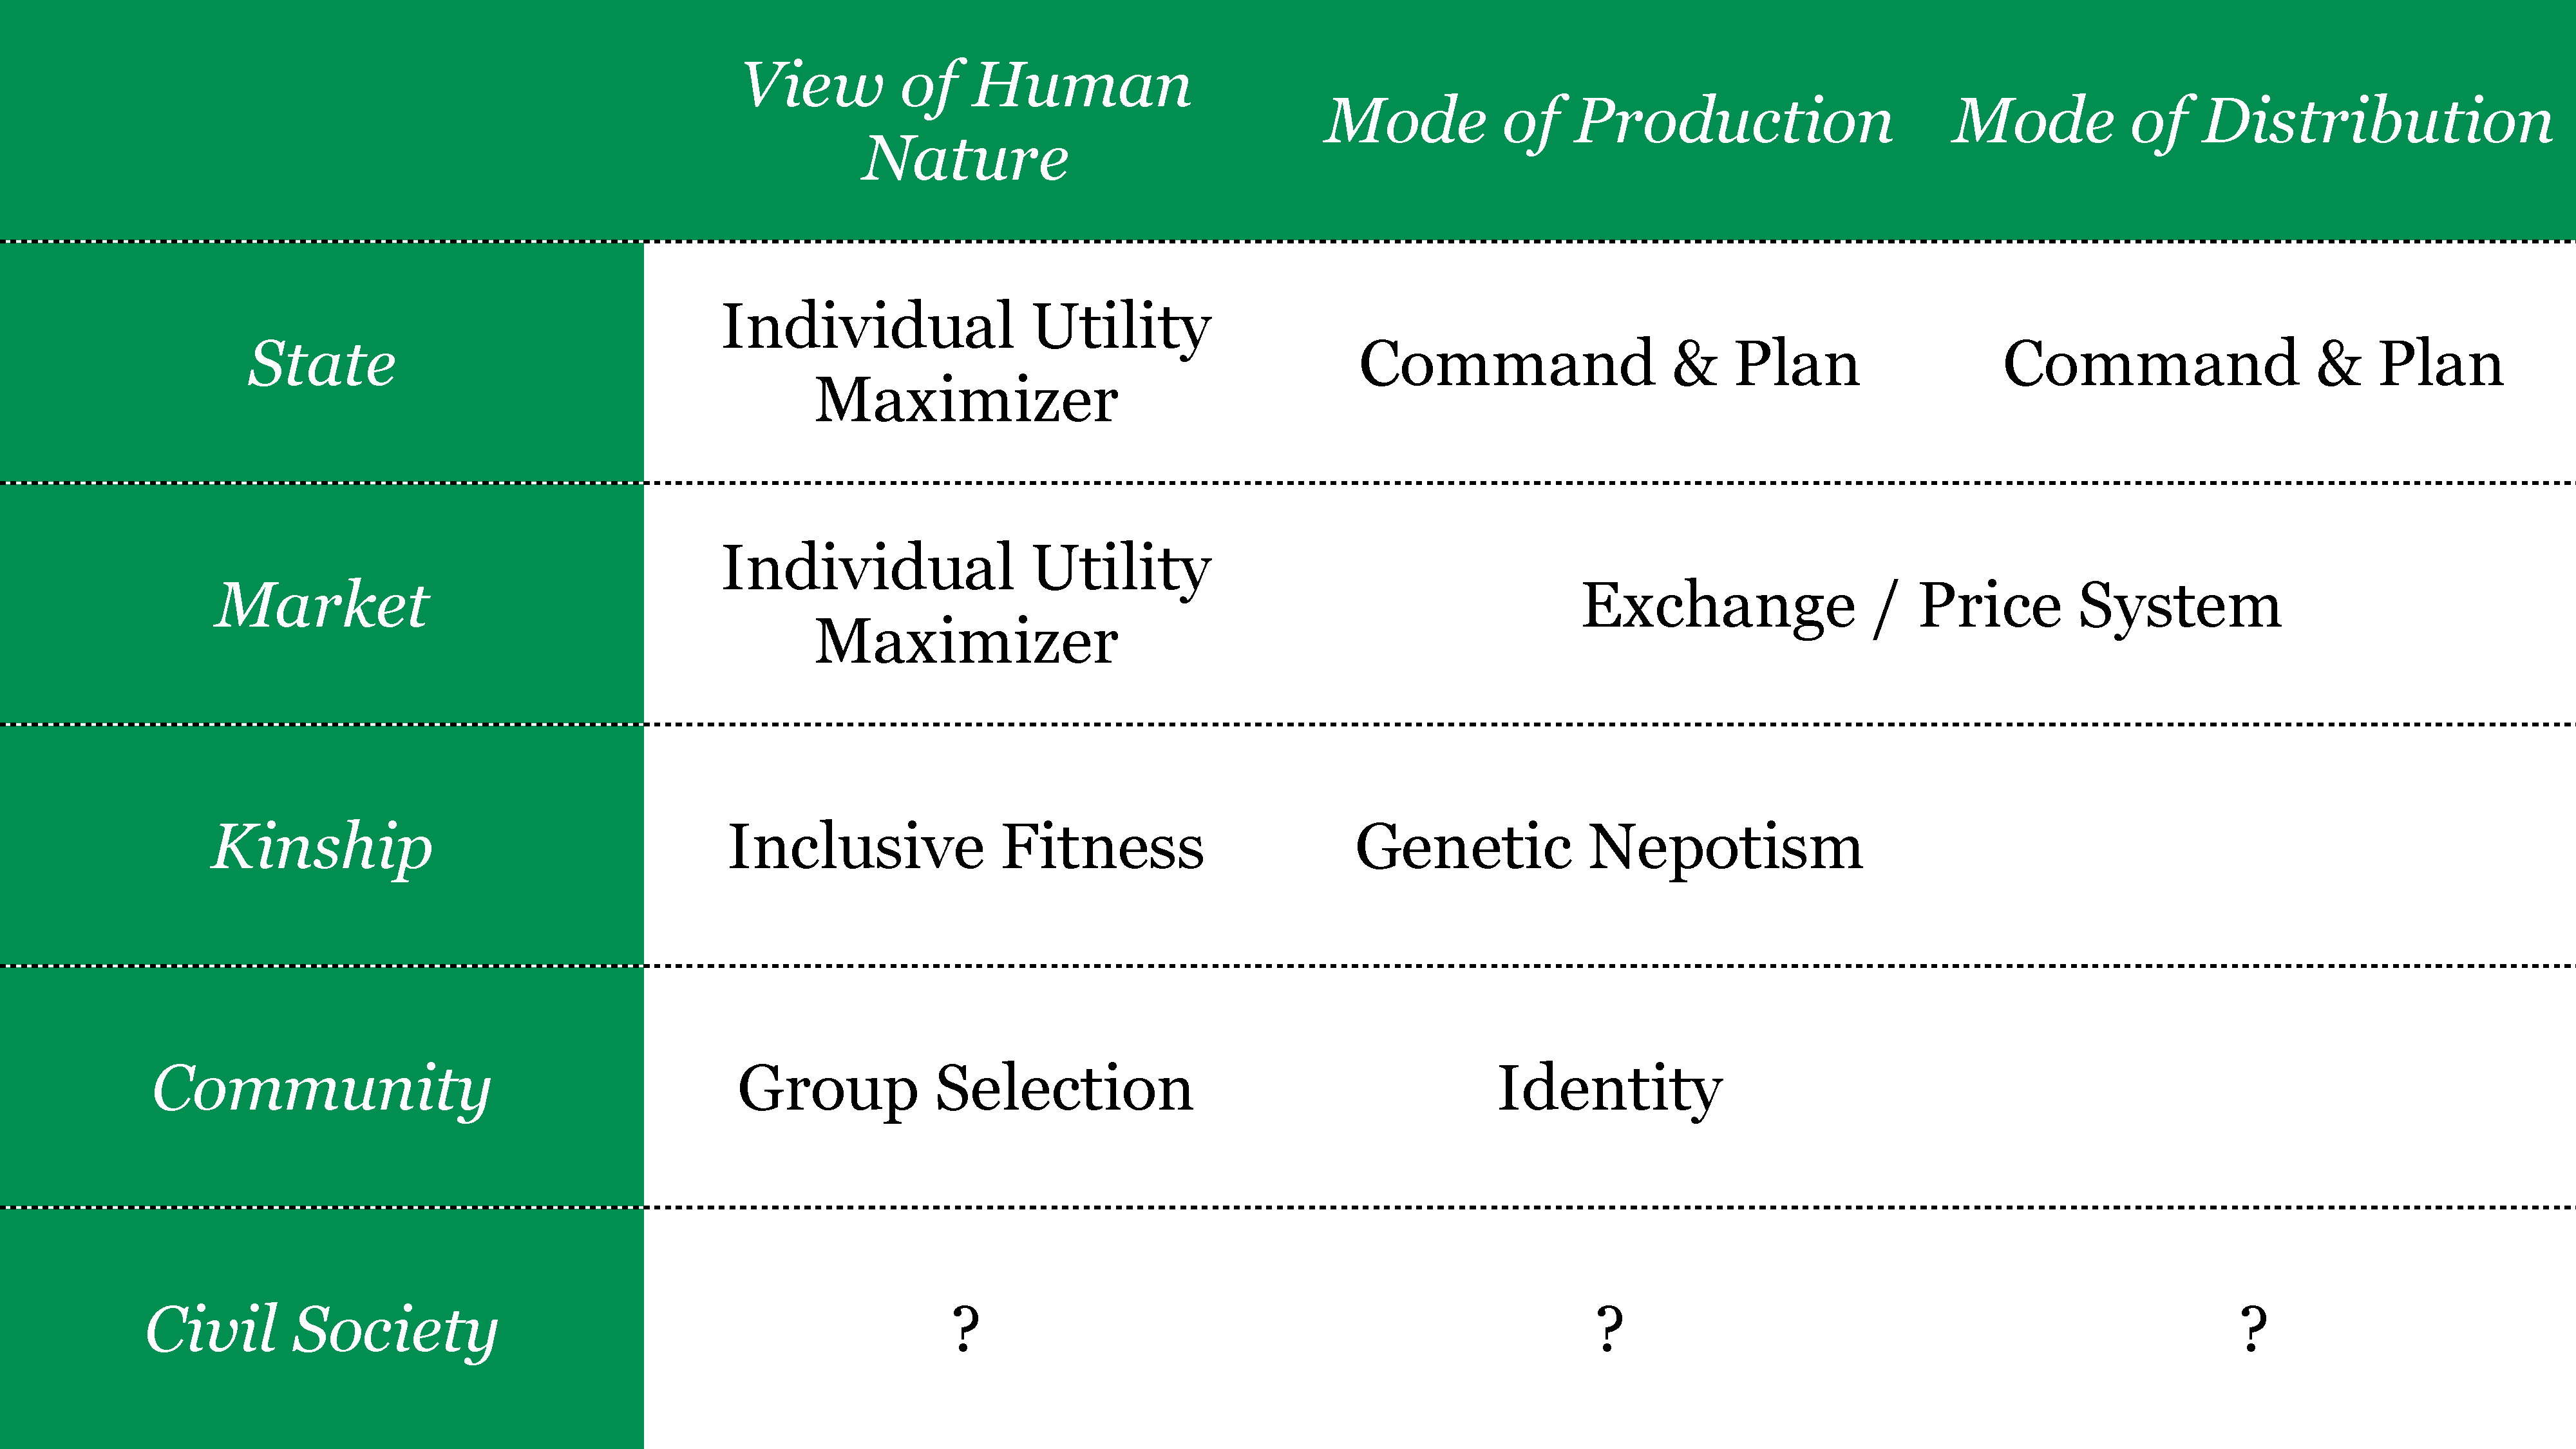
\includegraphics[width=1\linewidth]{modes-human-nature}
	\caption{Modes of Production, Distribution and Human Nature}
	\label{tab:modes-human-nature}
	\scriptsize{Own summary, but similar to \citealt[52f.]{Schmitter1985}}
\end{table}%remake this table in latex

At the economy or industry level, markets may be our best bet, but perhaps not at the firm or team level, where we can tap into other human motivations.
Similarly, a state may need to impose health and safety standards, but not a teacher's lesson plan (as \citeauthor{Schwartz2010} alarmingly report).
Market and state, along with their impoverished view of human nature, \emph{can} be applied selectively, to some domains.
As alternatives become available
\footnote{
	For example, the \gls{BIG} is a courageous suggestion to, among other things, decommodify \emph{and}, because it is no longer means-tested, ``de-regulate'' the livelihood \citep[for example,][]{Offe2009} and allow volunteerism.
},
market and state can recede
\footnote{
	As \citeauthor{Keynes} had promised:
	\begin{quote}
		\emph{``The day is not far off when the economic problem will take the back seat where it belongs, and the arena of the heart and the head will be occupied or reoccupied, by our real problems --- the problems of life and of human relations, of creation and behavior and religion.''}\\*
		--- John Maynard \cite{Keynes}%really, this is undated?
	\end{quote}
}.
For the time being, I suspect, the domains exclusive to market and state will remain considerable.

In this dissertation, I constrain homo economicus to the realm of the market, and summarize welfare and taxation policies to remedy, as well as make do with its shortcomings.
In democracy, by contrast, I find a realm in which homo economicus can no longer be accommodated, but where we must instead find new (deliberative) institutions to tap into other, better angels of our nature.
%add href

\subsubsection{No New Man}
Neither policy nor social scientific ontologies can ask for a \emph{new man}.
For better (see above) or for worse \citep[for example,][]{Schwartz2010}
\footnote{
	\cite{Schwartz2010} show how excessive regulation (the mode of states) and incentives (the mode of markets) can crowd out intrinsic motivation, ``Practical Wisdom'' and other, better angels of our nature.
	Unfortunately, this ship has probably sailed.
	Still, their insistence on a broader, human capacity to ``do well by doing good'' and crusade against dehumanizing choice is important.
}
state and market made their own humans:
as we live under hierarchy and competition, we adapt to it.
In the \gls{OECD}-world and in our time, many people (including me) will expect and respond to incentives and regulation.
Consequently, political institutions have to reckon with homo economicus, even if --- and because --- it is partly of their own making.

Good policy and good social scientific ontology does not ask for a new man, but makes do with the women and men we have now, but at the same time, recognizes that for our ``hypercultural'' species \citep{Henrich2004}, homo economicus, as other views on our indeterminate nature will always be highly \emph{contingent on institutions}.

None of this is to preclude a study or reform of human nature, modern society, states or markets.
Rather, such a contingent ontology is, to me, the \emph{only} way to study these meta-institutions and their incarnations in welfare, taxation and democracy.
\emph{Some}, ontologically contingent homo economicus can clear our hazy eyes, but \emph{too much}, ontologically endogenous homo economicus will blind our ``sociological imagination'' \citep{Mills-1959-aa}.
Contingency and domain-specificity lead the middle way between the hermetic ideology of utopias, and the apolitical mindlessness of \emph{TINAs}.

Also, none of this is to proclaim state and market as the ``end of history'' or to blazon homo economicus as ``the last man'' \citep{Fukuyama1992}.
Rather, state and market along with their homo economicus are the \emph{only} place to start from, if we want to write, or make history in welfare, taxation and democracy today.
Precisely because our nature is contingent on institutions, that is where we must start:
institutions are \emph{all we got}, ``just because institutions are the kinds of things that can can be changed directly, whereas cultures and psychological dispositions are less subject to collective intervention and experimentation'' \citep[K182]{WarrenPearse-2008-aa}.
States and markets are those prime meta-institutions through which we can make, and remake the institutions of welfare, taxation and democracy.
Through them, we respond to the homo economicus in all of us, and unfold our greater capacities.

And transcend the limits of homo economicus, we must.
Clearly, we face grave problems in \hyperref[chap:3-crises]{organizing production and distribution, and in reaching collective decisions} (\autoref{chap:3-crises}, p.~\pageref{chap:3-crises}).
Clearly, too, disintegration is not an option:
that way lies regress and hardship.
And clearly, further rational-functional or identity-embellished integration is not an option:
that way lie democratic deficits, and exclusionary identity politics.

These are the challenges cut out for us.
To fail them, to fail these cooperation problems of non-zero-sumness, is to fail specifically as a human being, the one ``conspicuously exceptional'' species \citep[85]{Frank2011} that is \emph{socially capable} of great cooperation, but not \emph{biologically determined} to give up individualism \citep{Wright2000}, and is therefore reliant on institutions.
Welfare, and especially taxation and democracy are those modern institutions, to square the circles of individuality, inequality and cooperation.

And these are the institutions I here assume to be malleable, to make up the desirable and doable hypotheticals, whose absence begs explanation.
These, too, are the institutions that moderate the very contingency of homo economicus, and our other natures.
As such, they are precisely the place to look at, taking on one second-order question at a time, leaving all else to first-order status.

For sociology, ``the science of institutions, their genesis and their functioning'' \citep[45]{Durkheim1895}, this, I would hope, is a good approach as any to learn --- as we must --- whether, and under which (institutional!) circumstances humans are ``knights, knaves, pawns or queens'' \citep{LeGrand2003}, what our capacity for altruism is \citep{Henrich2007} and how it can be fostered \citep{Axelrod1981a}, all to imagine, and then fulfill our human capacity of non-zero-sumness \citep{Wright2000}.